\chapter{Preliminary work}
	\label{sec:preliminary-work}
	
	% TODO: Add more linking together perhaps?
	
	The preliminary work outlined in this chapter initially concentrates on
	developing a fuller understanding of the characteristics of the
	interconnection networks used in SpiNNaker. This work has developed into the
	foundations for new extensions to the SpiNNaker network which will form the
	main contributions of this project.
	
	The chapter begins with the development of an efficient wiring scheme for
	large SpiNNaker systems which accounts for the properties of HSS interconnect
	technology. This is followed by a discussion of an extension to the network
	which exploits this wiring scheme to inexpensively transform the network into
	a small world network with improved latency.  As part of an effort to validate
	potential changes to the network, a model of SpiNNaker's interconnection
	network has been built. A brief description of this work is included along
	with details of collaborative work to develop new modelling techniques.  The
	chapter concludes with an overview of extensions being made to the existing
	HSS board-to-board links within SpiNNaker which will form the foundations of
	an implementation of small world networking.
	
	\section{SpiNNaker machine wiring}
		
		% Constraint of electrical high-speed-serial is that long wires are not
		% allowed. For tori, this is a problem due to wrap-around.
		
		Electrical HSS links impose restrictions on the maximum length of cables. In
		the case of SpiNNaker's board-to-board links, which follow the S-ATA
		physical connection standard, cable lengths are limited to one meter for
		most applications \cite{sata3spec}. Due to SpiNNaker's torus topology, this
		restriction necessitates a non-trivial wiring scheme as described in this
		section.
		
		\begin{figure}
			\center
			\input{|"python2 figures/boardsLogical.py"}
			\caption[Logical arrangement of boards in a 48 board SpiNNaker
			system.]{Logical arrangement of boards in a 48 board SpiNNaker system.
			Touching boards are connected. Coloured lines represent long connections
			travelling {\color{red}North/South},
			{\color{green}North-East/South-West} and {\color{blue}East/West}.}
			\label{fig:boardsLogical}
		\end{figure}
		
		Figure \ref{fig:boardsLogical} shows the logical connectivity between boards
		in a small SpiNNaker system containing 48 boards (represented as hexagons).
		Touching edges represent a connection between two boards. Lines show the
		connectivity between boards on opposite sides of the system. While the
		majority of wires are very short (i.e. connect two boards which are
		side-by-side), some wires must cross the entire system's length. If
		SpiNNaker boards are arranged na\"ively to match their logical layout, for
		the largest planned SpiNNaker machine, spanning ten server-room cabinets,
		wires over six meters long would be needed, far beyond the one metre
		technology limit.
		
		The principles of the machine's construction described by by Davidson
		\cite{davidsonWiring} and Furber \cite{furber13email} were used as the basis
		for a tool, SpiNNer, used to model and experiment with possible physical
		arrangements of SpiNNaker boards \footnote{The SpiNNer tool was also used to
		generate many of the figures in this section.}. The development and use of
		this tool has led to the design of practical wiring schemes for SpiNNaker
		systems ranging in size from three boards to a ten cabinets (1,200 boards).
		This section describes the principle by which these schemes are produced.
		
		\subsection{Reducing wiring length}
			
			\begin{figure}
				\begin{subfigure}[b]{\textwidth}
					\center
					\begin{tikzpicture}[thick,inner sep=0.1cm]
	\node [fill,circle] (node 153942796) at (0.000000,0.000000) {};
	\node [fill,circle] (node 160312652) at (1.000000,0.000000) {};
	\node [fill,circle] (node 160312684) at (2.000000,0.000000) {};
	\node [fill,circle] (node 160312716) at (3.000000,0.000000) {};
	\node [fill,circle] (node 160312812) at (4.000000,0.000000) {};
	\node [fill,circle] (node 160312908) at (5.000000,0.000000) {};
	\node [fill,circle] (node 160313036) at (6.000000,0.000000) {};
	\node [fill,circle] (node 160313164) at (7.000000,0.000000) {};
	\node [fill,circle] (node 160313292) at (8.000000,0.000000) {};
	\node [fill,circle] (node 160444524) at (9.000000,0.000000) {};
	\node [fill,circle] (node 160444652) at (10.000000,0.000000) {};
	\node [fill,circle] (node 160444812) at (11.000000,0.000000) {};
	
	\draw (node 153942796)
							         .. controls +(-1.000000,0.500000)
							                 and +(1.000000,0.500000)
							         .. (node 160444812);
	\draw (node 153942796) -- (node 160312652);
	\draw (node 160312652) -- (node 160312684);
	\draw (node 160312684) -- (node 160312716);
	\draw (node 160312716) -- (node 160312812);
	\draw (node 160312812) -- (node 160312908);
	\draw (node 160312908) -- (node 160313036);
	\draw (node 160313036) -- (node 160313164);
	\draw (node 160313164) -- (node 160313292);
	\draw (node 160313292) -- (node 160444524);
	\draw (node 160444524) -- (node 160444652);
	\draw (node 160444652) -- (node 160444812);
\end{tikzpicture}

					\caption{A ring network}
					\label{fig:ringLong}
				\end{subfigure}
				
				\vspace{2ex}
				
				\begin{subfigure}[b]{\textwidth}
					\center
					\begin{tikzpicture}[thick,inner sep=0.1cm]
	\node [fill,circle] (node 151878444) at (0.000000,0.000000) {};
	\node [fill,circle] (node 158252396) at (2.000000,0.000000) {};
	\node [fill,circle] (node 158252428) at (4.000000,0.000000) {};
	\node [fill,circle] (node 158252460) at (6.000000,0.000000) {};
	\node [fill,circle] (node 158252556) at (8.000000,0.000000) {};
	\node [fill,circle] (node 158252652) at (10.000000,0.000000) {};
	\node [fill,circle] (node 158252780) at (11.000000,0.500000) {};
	\node [fill,circle] (node 158252908) at (9.000000,0.500000) {};
	\node [fill,circle] (node 158253036) at (7.000000,0.500000) {};
	\node [fill,circle] (node 158384268) at (5.000000,0.500000) {};
	\node [fill,circle] (node 158384396) at (3.000000,0.500000) {};
	\node [fill,circle] (node 158384556) at (1.000000,0.500000) {};
	
	\draw (node 151878444) -- (node 158384556);
	\draw (node 151878444) -- (node 158252396);
	\draw (node 158252396) -- (node 158252428);
	\draw (node 158252428) -- (node 158252460);
	\draw (node 158252460) -- (node 158252556);
	\draw (node 158252556) -- (node 158252652);
	\draw (node 158252652) -- (node 158252780);
	\draw (node 158252780) -- (node 158252908);
	\draw (node 158252908) -- (node 158253036);
	\draw (node 158253036) -- (node 158384268);
	\draw (node 158384268) -- (node 158384396);
	\draw (node 158384396) -- (node 158384556);
\end{tikzpicture}

					\caption{Folded in half}
					\label{fig:ringFolded}
				\end{subfigure}
				
				\vspace{2ex}
				
				\begin{subfigure}[b]{\textwidth}
					\center
					\begin{tikzpicture}[thick,inner sep=0.1cm]
	\node [fill,circle] (node 155478860) at (0.000000,0.000000) {};
	\node [fill,circle] (node 161861004) at (2.000000,0.000000) {};
	\node [fill,circle] (node 161861036) at (4.000000,0.000000) {};
	\node [fill,circle] (node 161861068) at (6.000000,0.000000) {};
	\node [fill,circle] (node 161861164) at (8.000000,0.000000) {};
	\node [fill,circle] (node 161861260) at (10.000000,0.000000) {};
	\node [fill,circle] (node 161861388) at (11.000000,0.000000) {};
	\node [fill,circle] (node 161861516) at (9.000000,0.000000) {};
	\node [fill,circle] (node 161988652) at (7.000000,0.000000) {};
	\node [fill,circle] (node 161988780) at (5.000000,0.000000) {};
	\node [fill,circle] (node 161988908) at (3.000000,0.000000) {};
	\node [fill,circle] (node 161989068) at (1.000000,0.000000) {};
	
	\draw (node 155478860) -- (node 161989068);
	\draw (node 155478860)
							         .. controls +(1.000000,0.500000)
							                 and +(-1.000000,0.500000)
							         .. (node 161861004);
	\draw (node 161861004)
							         .. controls +(1.000000,0.500000)
							                 and +(-1.000000,0.500000)
							         .. (node 161861036);
	\draw (node 161861036)
							         .. controls +(1.000000,0.500000)
							                 and +(-1.000000,0.500000)
							         .. (node 161861068);
	\draw (node 161861068)
							         .. controls +(1.000000,0.500000)
							                 and +(-1.000000,0.500000)
							         .. (node 161861164);
	\draw (node 161861164)
							         .. controls +(1.000000,0.500000)
							                 and +(-1.000000,0.500000)
							         .. (node 161861260);
	\draw (node 161861260) -- (node 161861388);
	\draw (node 161861388)
							         .. controls +(-1.000000,0.500000)
							                 and +(1.000000,0.500000)
							         .. (node 161861516);
	\draw (node 161861516)
							         .. controls +(-1.000000,0.500000)
							                 and +(1.000000,0.500000)
							         .. (node 161988652);
	\draw (node 161988652)
							         .. controls +(-1.000000,0.500000)
							                 and +(1.000000,0.500000)
							         .. (node 161988780);
	\draw (node 161988780)
							         .. controls +(-1.000000,0.500000)
							                 and +(1.000000,0.500000)
							         .. (node 161988908);
	\draw (node 161988908)
							         .. controls +(-1.000000,0.500000)
							                 and +(1.000000,0.500000)
							         .. (node 161989068);
\end{tikzpicture}

					\caption{Interleaved}
					\label{fig:ringInterleaved}
				\end{subfigure}
				
				\caption[Folding a ring network.]{The process of folding a ring network
				to reduce the maximum wire length.}
				\label{fig:folding}
			\end{figure}
			
			\begin{figure}
				\center
				\begin{subfigure}[b]{\textwidth}
					\center
					\input{|"python2 figures/boardsFoldedShift.py"}
					\caption{Shift boards on the left to the right to form a rectangle.}
					\label{fig:boardsFoldedShift}
				\end{subfigure}
				
				\vspace{2ex}
				
				\begin{subfigure}[b]{\textwidth}
					\center
					\input{|"python2 figures/boardsFoldedSpaced.py"}
					\caption{Fold along the gaps in this figure. (Wires omitted for
					clarity.)}
					\label{fig:boardsFoldedSpaced}
				\end{subfigure}
				
				\vspace{2ex}
				
				\begin{subfigure}[b]{\textwidth}
					\center
					\input{|"python2 figures/boardsFoldedInterleaved.py"}
					\caption{The (more complex) wiring after folding. (Shown here with
					squares since hexagons do not visually fit together after folding and
					interleaving.)}
					\label{fig:boardsFoldedInterleaved}
				\end{subfigure}
				
				\caption[Folding SpiNNaker.]{The process of folding SpiNNaker. Coloured
				lines represent wires travelling {\color{red}North/South},
				{\color{green}North-East/South-West} and {\color{blue}East/West}.}
				\label{fig:boardsFolded}
			\end{figure}
			
			Long wires can be avoided in toroidal networks by `folding'
			\cite{dally04}.  An example of this process is shown for a simple
			ring-network (a 1-dimensional toroid) in figure \ref{fig:folding}. This
			process is generalised to SpiNNaker's boards as shown in figure
			\ref{fig:boardsFolded}. The first step (figure
			\ref{fig:boardsFoldedShift}) transforms the rhombus-like arrangement of
			boards into a rectangle which is more easily folded.
			
			In the next step, the design is folded into four parts along the Y-axis
			and into two along the X-axis (figure \ref{fig:boardsFoldedSpaced}). It is
			necessary to fold along the Y-axis into four to eliminate the long,
			diagonal connections. Folding in two would not bring these points any
			closer while folding into four brings them next to each other. For
			example, the wire travelling from the bottom left board to the top-middle
			board after folding in two would now have to cross from one end of the
			system to the other, an even longer distance than it had to before. By
			folding in this way the maximum wire length is reduced producing the
			wiring shown in figure \ref{fig:boardsFoldedInterleaved}.
			
			\label{sec:mapping-spinnaker-to-cabinets}
			
			\begin{figure}
				\center
				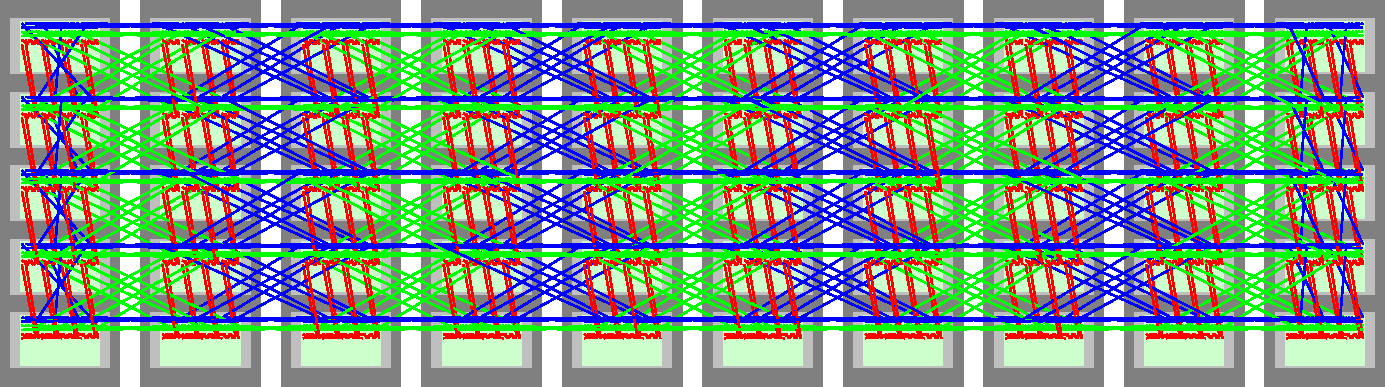
\includegraphics[width=\textwidth]{figures/spinnaker106}
				\caption[SpiNNaker machine mapped into cabinets and racks.]{The largest
				planned SpiNNaker machine with 1,200 boards and 1,036,800 cores mapped
				into 10 cabinets of 5 racks each.  Coloured lines represent wires
				connecting {\color{red}North/South},
				{\color{green}North-East/South-West} and {\color{blue}East/West} links.}
				\label{fig:spinnaker106}
			\end{figure}
			
			The final step in the process is to map the boards into their real-world
			physical positions. The largest SpiNNaker system will be installed into a
			series of cabinets, each containing a number of racks into which the
			boards are slotted and wired together. Figure \ref{fig:spinnaker106} shows
			the proposed rack placement scheme for the largest planned SpiNNaker
			system of 1,200 boards. Even though the system is physically around six
			metres long, the longest wire will be less than one metre in length and
			thus within the S-ATA specification.
		
		\subsection{Future Work}
			
			% The tool has been successfuly used to
			% assemble machines (pictures!) and provide orders for cabling for the
			% next machines. Next stage will involve extending this to interactively
			% guiding larger builds and 
			
			\begin{figure}
				\begin{subfigure}{0.49\textwidth}
					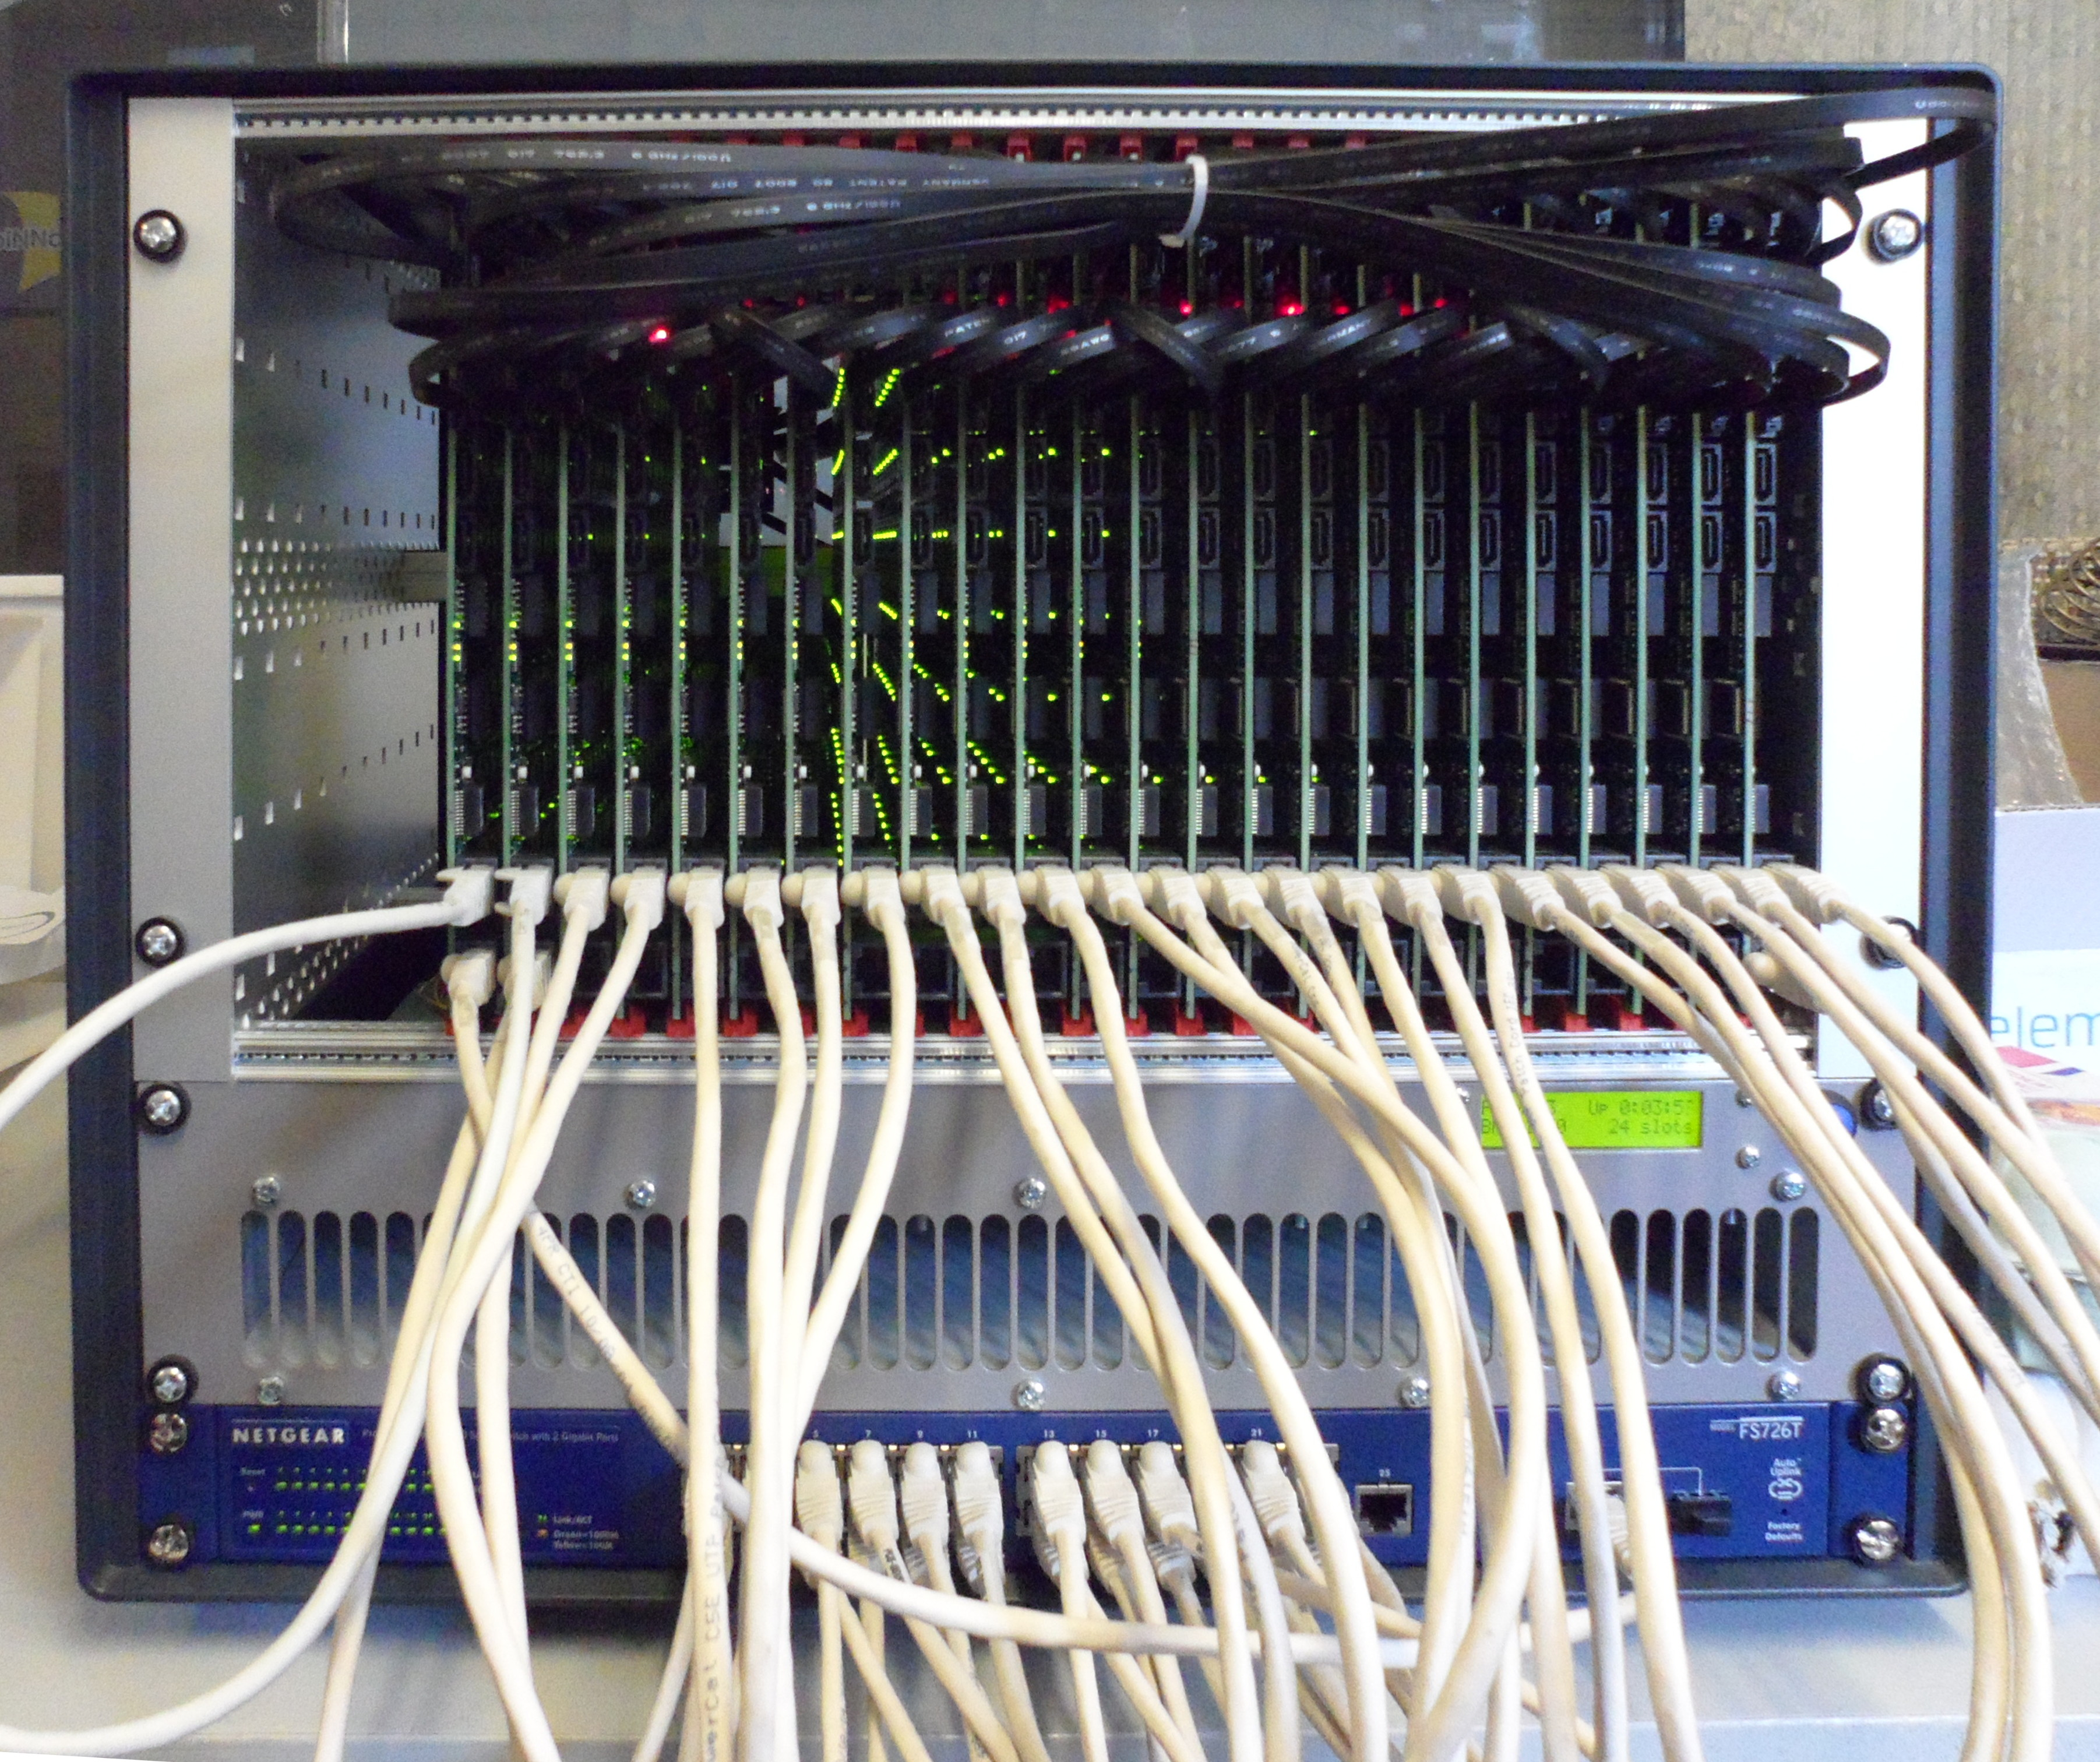
\includegraphics[width=\textwidth]{figures/rack-front.jpg}
					
					\caption{Front}
					\label{fig:rack-front}
				\end{subfigure}
				\begin{subfigure}{0.49\textwidth}
					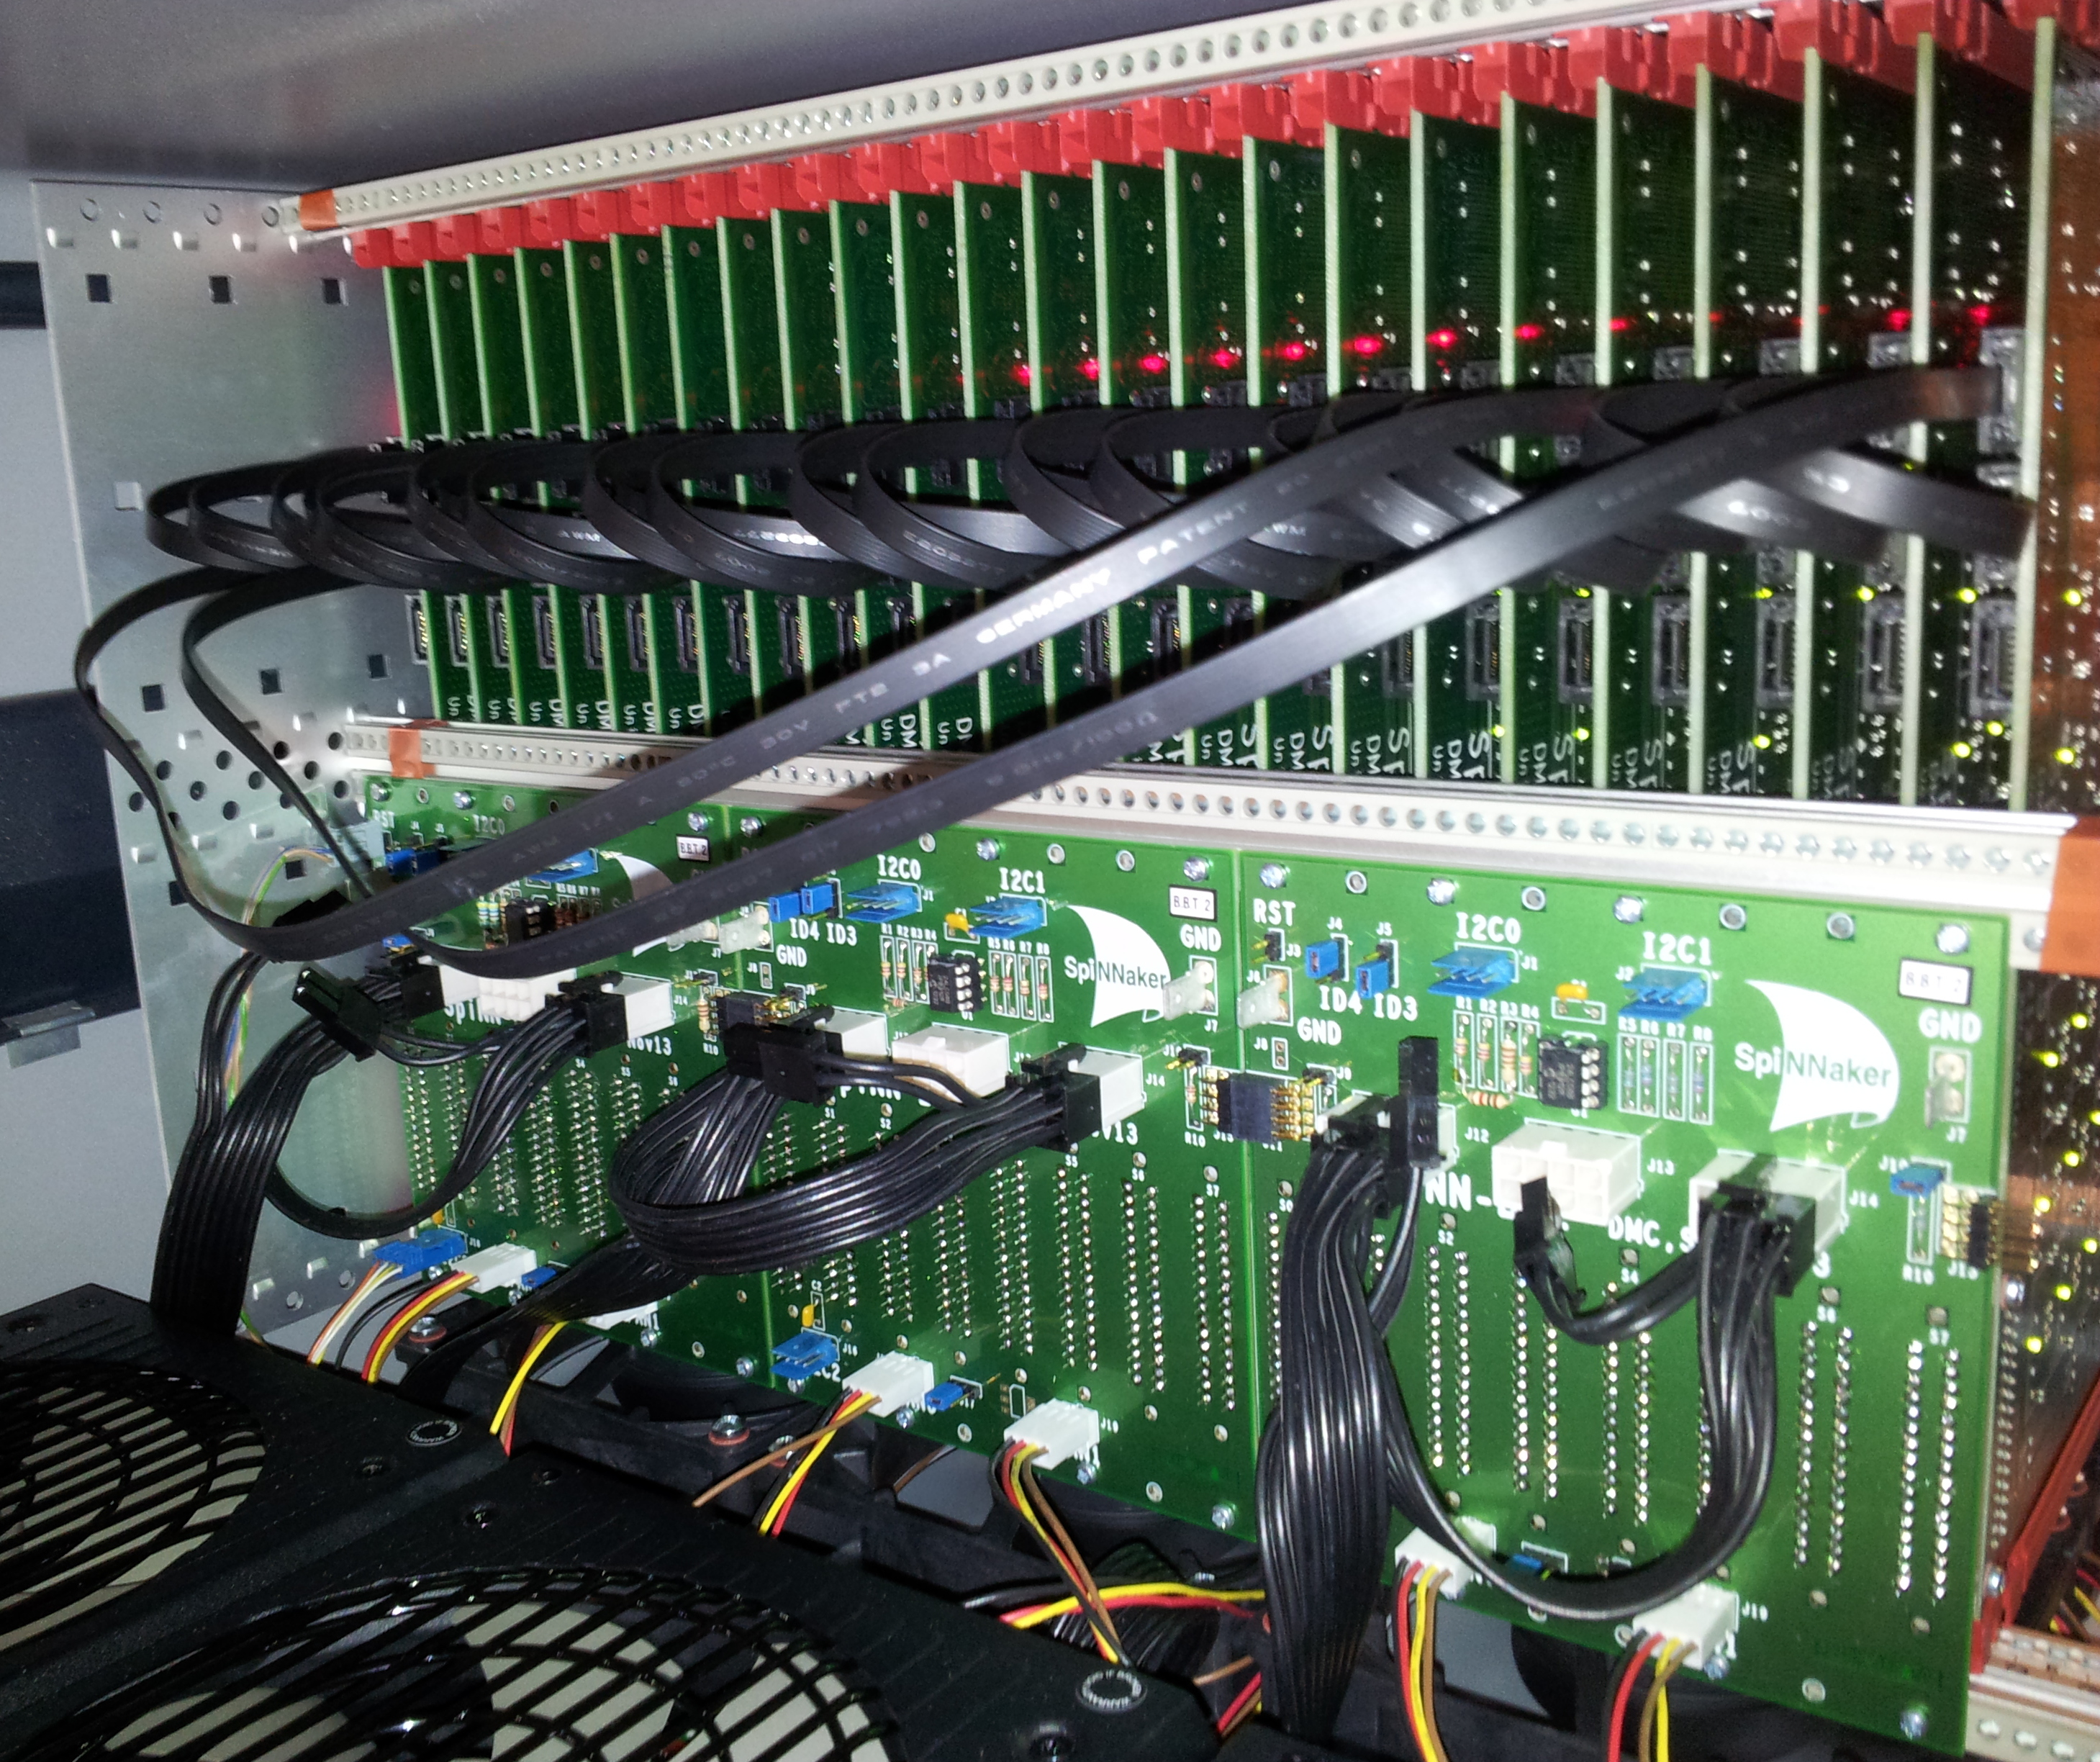
\includegraphics[width=\textwidth]{figures/rack-back.jpg}
					
					\caption{Back}
					\label{fig:rack-back}
				\end{subfigure}
				
				\caption{Wiring for a prototype `desk-side' SpiNNaker system.}
				\label{fig:rack}
			\end{figure}
			
			Wiring plans produced by SpiNNer have already successfully been used in
			the construction of small `desk-side' 24-board SpiNNaker systems
			containing 20,736 cores (figure \ref{fig:rack}. The tool is also being
			used in the ongoing construction of larger SpiNNaker machines. Due to the
			larger size of these machines, the tool must be extended to break down
			wiring diagrams into multiple diagrams to aid usability.
	
	
	\section{Small-world networks}
		
		% Small world networks are: ... Allow lots of short paths, this means low
		% latency, low power and less contention. We describe ways of augmenting the
		% SpiNNaker network, making use of spare connections and resource for
		% board-to-board links while taking advantage of the physical arrangement
		% described in the previous section.
		
		Small-world networks are graphs with a very large number of nodes but,
		within which, the shortest path between any pair of nodes is small.
		Additionally, each node in the graph features only a relatively small number
		of connections. They also contain `clusters' of well connected nodes, in
		contrast with random graphs (which may also fulfil the first criterion).
		
		Small world networks are often found in nature, perhaps most famously in
		social networks. In this context, the phenomenon was first observed in 1929
		by Hungarian author Frigyes Karinthy\cite{karinthy29} and the idea has
		become popularly known as the theory of `six degrees of separation'. The
		theory states that for any two people on earth, chosen at random, there is a
		chain of at most 6 acquaintances which connects them.
		
		This property of maintaining low maximum shortest-path length while still
		remaining locally well connected is desirable for certain computational
		problems. In neural simulations, most communication is local with just a few
		longer connections. The clustering property of small world networks means
		these local connections can be well catered for while the low maximum
		shortest-path length means longer connections are still quick for very large
		models.
		
		In this section a method for constructing small-world networks within
		SpiNNaker's board-to-board links is introduced which does not require
		physically long connections while still exhibiting significant reductions in
		network latency.
		
		\subsection{Constructing small-world networks}
			
			% Add random links and lo-and-behold, smallworldness!
			
			Watts and Strogatz have proposed an algorithm for randomly constructing
			networks with small-world properties \cite{watts98}. The algorithm begins
			by creating a ring-like network with each node connecting to a fixed
			number of its neighbours (figure \ref{fig:ringNetworkB0}). In the next
			step, with a probability of $\beta$, each edge may be replaced by a random
			connection.  For $0 < \beta < 1$, the networks produced exhibit varying
			degrees of the small-world properties (figure \ref{fig:ringNetworkB02}).
			Finally, in the extreme case where $\beta=1$, the network devolves into a
			random network (figure \ref{fig:ringNetworkB1}).
			
			\begin{figure}
				\center
				\begin{subfigure}[t]{0.3\textwidth}
					\center
					\begin{tikzpicture}[thick,inner sep=0.1cm]
	\foreach \t in {30,60,...,360}{
		\node [fill,circle] at (\t:2) {};
		\draw (\t:2) -- (\t+30:2);
		\draw (\t:2) -- (\t+60:2);
	}
\end{tikzpicture}


					\caption{Ring ($\beta = 0.0$)}
					\label{fig:ringNetworkB0}
				\end{subfigure}
				\begin{subfigure}[t]{0.3\textwidth}
					\center
					\newcommand{\mayberandompath}[2]{
	\pgfmathsetmacro{\choice}{random(5)}
	\pgfmathsetmacro{\myrand}{random(12)*30}
	\ifthenelse{\equal{\choice}{1.0}}{
		\draw (#1:2) -- (#2+\myrand:2);
	}{
		\draw (#1:2) -- (#2:2);
	}
}

\begin{tikzpicture}[thick,inner sep=0.1cm]
	\foreach \t in {30,60,...,360}{
		\node [fill,circle] at (\t:2) {};
		\mayberandompath{\t}{\t+30}
		\mayberandompath{\t}{\t+60}
	}
\end{tikzpicture}

					\caption{Watts-Strogatz ($\beta = 0.2$)}
					\label{fig:ringNetworkB02}
				\end{subfigure}
				\begin{subfigure}[t]{0.3\textwidth}
					\center
					\newcommand{\mayberandompath}[2]{
	\pgfmathsetmacro{\myrand}{random(12)*30}
	\draw (#1:2) -- (#2+\myrand:2);
}

\begin{tikzpicture}[thick,inner sep=0.1cm]
	\foreach \t in {30,60,...,360}{
		\node [fill,circle] at (\t:2) {};
		\mayberandompath{\t}{\t+30}
		\mayberandompath{\t}{\t+60}
	}
	
\end{tikzpicture}

					\caption{Random ($\beta = 1.0$)}
					\label{fig:ringNetworkB1}
				\end{subfigure}
				
				\caption{Watts-Strogatz networks with a range of rewiring
				probabilities.}
				\label{fig:ringNetwork}
			\end{figure}
		
		\subsection{Modelling and results}
			
			% Don't need too many links to get a good return in terms of reduced
			% path length. Limiting results to short wires doesn't hurt too much,
			% especially after folding.
			
			\begin{figure}
				\center
				\begin{subfigure}[t]{0.45\textwidth}
					\center
					\begin{tikzpicture}[thick,inner sep=0.1cm]
	\clip (-0.5,-0.5) rectangle (5.5,5.5);
	
	\node [fill,circle] (node 146024940) at (0,0) {};
	\node [fill,circle] (node 152407084) at (1,0) {};
	\node [fill,circle] (node 152406988) at (2,0) {};
	\node [fill,circle] (node 152407180) at (3,0) {};
	\node [fill,circle] (node 152407276) at (4,0) {};
	\node [fill,circle] (node 152407404) at (5,0) {};
	\node [fill,circle] (node 152407564) at (0,1) {};
	\node [fill,circle] (node 152407692) at (1,1) {};
	\node [fill,circle] (node 152407724) at (2,1) {};
	\node [fill,circle] (node 152407788) at (3,1) {};
	\node [fill,circle] (node 152407820) at (4,1) {};
	\node [fill,circle] (node 152407948) at (5,1) {};
	\node [fill,circle] (node 152531052) at (0,2) {};
	\node [fill,circle] (node 152531148) at (1,2) {};
	\node [fill,circle] (node 152531180) at (2,2) {};
	\node [fill,circle] (node 152531212) at (3,2) {};
	\node [fill,circle] (node 152531276) at (4,2) {};
	\node [fill,circle] (node 152537548) at (5,2) {};
	\node [fill,circle] (node 152553292) at (0,3) {};
	\node [fill,circle] (node 152553836) at (1,3) {};
	\node [fill,circle] (node 152554092) at (2,3) {};
	\node [fill,circle] (node 152554668) at (3,3) {};
	\node [fill,circle] (node 152554892) at (4,3) {};
	\node [fill,circle] (node 152580172) at (5,3) {};
	\node [fill,circle] (node 152580940) at (0,4) {};
	\node [fill,circle] (node 152581804) at (1,4) {};
	\node [fill,circle] (node 152610924) at (2,4) {};
	\node [fill,circle] (node 152609420) at (3,4) {};
	\node [fill,circle] (node 152656748) at (4,4) {};
	\node [fill,circle] (node 152656844) at (5,4) {};
	\node [fill,circle] (node 152656972) at (0,5) {};
	\node [fill,circle] (node 152657068) at (1,5) {};
	\node [fill,circle] (node 152657100) at (2,5) {};
	\node [fill,circle] (node 152657132) at (3,5) {};
	\node [fill,circle] (node 152657164) at (4,5) {};
	\node [fill,circle] (node 152657260) at (5,5) {};
	
	\draw (node 146024940)
							         .. controls +(0.500000,-1.000000)
							                 and +(0.500000,1.000000)
							         .. (node 152656972);
	\draw (node 146024940)
							         .. controls +(-1.000000,0.500000)
							                 and +(1.000000,0.500000)
							         .. (node 152407404);
	\draw (node 146024940) -- (node 152407084);
	\draw (node 146024940) -- (node 152407564);
	\draw (node 152407084) -- (node 152407692);
	\draw (node 152407084)
							         .. controls +(0.500000,-1.000000)
							                 and +(0.500000,1.000000)
							         .. (node 152657068);
	\draw (node 152406988) -- (node 152407180);
	\draw (node 152406988) -- (node 152407724);
	\draw (node 152406988) -- (node 152407084);
	\draw (node 152406988)
							         .. controls +(0.500000,-1.000000)
							                 and +(0.500000,1.000000)
							         .. (node 152657100);
	\draw (node 152407180)
							         .. controls +(0.500000,-1.000000)
							                 and +(0.500000,1.000000)
							         .. (node 152657132);
	\draw (node 152407180) -- (node 152407276);
	\draw (node 152407180) -- (node 152407788);
	\draw (node 152407276) -- (node 152407404);
	\draw (node 152407276) -- (node 152407820);
	\draw (node 152407276)
							         .. controls +(0.500000,-1.000000)
							                 and +(0.500000,1.000000)
							         .. (node 152657164);
	\draw (node 152407404) -- (node 152407948);
	\draw (node 152407404)
							         .. controls +(0.500000,-1.000000)
							                 and +(0.500000,1.000000)
							         .. (node 152657260);
	\draw (node 152407564)
							         .. controls +(-1.000000,0.500000)
							                 and +(1.000000,0.500000)
							         .. (node 152407948);
	\draw (node 152407564) -- (node 152531052);
	\draw (node 152407564) -- (node 152407692);
	\draw (node 152407692) -- (node 152407724);
	\draw (node 152407692) -- (node 152531148);
	\draw (node 152407724) -- (node 152407788);
	\draw (node 152407724) -- (node 152531180);
	\draw (node 152407788) -- (node 152407820);
	\draw (node 152407788) -- (node 152531212);
	\draw (node 152407820) -- (node 152531276);
	\draw (node 152407820) -- (node 152407948);
	\draw (node 152407948) -- (node 152537548);
	\draw (node 152531052) -- (node 152553292);
	\draw (node 152531052)
							         .. controls +(-1.000000,0.500000)
							                 and +(1.000000,0.500000)
							         .. (node 152537548);
	\draw (node 152531052) -- (node 152531148);
	\draw (node 152531148) -- (node 152553836);
	\draw (node 152531148) -- (node 152531180);
	\draw (node 152531180) -- (node 152554092);
	\draw (node 152531180) -- (node 152531212);
	\draw (node 152531212) -- (node 152531276);
	\draw (node 152531212) -- (node 152554668);
	\draw (node 152531276) -- (node 152537548);
	\draw (node 152531276) -- (node 152554892);
	\draw (node 152537548) -- (node 152580172);
	\draw (node 152553292) -- (node 152580940);
	\draw (node 152553292)
							         .. controls +(-1.000000,0.500000)
							                 and +(1.000000,0.500000)
							         .. (node 152580172);
	\draw (node 152553292) -- (node 152553836);
	\draw (node 152553836) -- (node 152554092);
	\draw (node 152553836) -- (node 152581804);
	\draw (node 152554092) -- (node 152610924);
	\draw (node 152554092) -- (node 152554668);
	\draw (node 152554668) -- (node 152554892);
	\draw (node 152554668) -- (node 152609420);
	\draw (node 152554892) -- (node 152580172);
	\draw (node 152554892) -- (node 152656748);
	\draw (node 152580172) -- (node 152656844);
	\draw (node 152580940)
							         .. controls +(-1.000000,0.500000)
							                 and +(1.000000,0.500000)
							         .. (node 152656844);
	\draw (node 152580940) -- (node 152656972);
	\draw (node 152580940) -- (node 152581804);
	\draw (node 152581804) -- (node 152610924);
	\draw (node 152581804) -- (node 152657068);
	\draw (node 152610924) -- (node 152657100);
	\draw (node 152609420) -- (node 152656748);
	\draw (node 152609420) -- (node 152610924);
	\draw (node 152609420) -- (node 152657132);
	\draw (node 152656748) -- (node 152656844);
	\draw (node 152656748) -- (node 152657164);
	\draw (node 152656844) -- (node 152657260);
	\draw (node 152656972)
							         .. controls +(-1.000000,0.500000)
							                 and +(1.000000,0.500000)
							         .. (node 152657260);
	\draw (node 152656972) -- (node 152657068);
	\draw (node 152657068) -- (node 152657100);
	\draw (node 152657100) -- (node 152657132);
	\draw (node 152657132) -- (node 152657164);
	\draw (node 152657164) -- (node 152657260);
\end{tikzpicture}

					\caption{Unmodified torus ($\beta=0.0$)}
					\label{fig:torusNetworkB0}
				\end{subfigure}
				\begin{subfigure}[t]{0.45\textwidth}
					\center
					\begin{tikzpicture}[thick,inner sep=0.1cm]
	\clip (-0.5,-0.5) rectangle (5.5,5.5);
	
	\node [fill,circle] (node 163015180) at (0,0) {};
	\node [fill,circle] (node 169393228) at (1,0) {};
	\node [fill,circle] (node 169393132) at (2,0) {};
	\node [fill,circle] (node 169393324) at (3,0) {};
	\node [fill,circle] (node 169393420) at (4,0) {};
	\node [fill,circle] (node 169393548) at (5,0) {};
	\node [fill,circle] (node 169393708) at (0,1) {};
	\node [fill,circle] (node 169393836) at (1,1) {};
	\node [fill,circle] (node 169393868) at (2,1) {};
	\node [fill,circle] (node 169393932) at (3,1) {};
	\node [fill,circle] (node 169393964) at (4,1) {};
	\node [fill,circle] (node 169394092) at (5,1) {};
	\node [fill,circle] (node 169521292) at (0,2) {};
	\node [fill,circle] (node 169521388) at (1,2) {};
	\node [fill,circle] (node 169521420) at (2,2) {};
	\node [fill,circle] (node 169521452) at (3,2) {};
	\node [fill,circle] (node 169521516) at (4,2) {};
	\node [fill,circle] (node 169527788) at (5,2) {};
	\node [fill,circle] (node 169543532) at (0,3) {};
	\node [fill,circle] (node 169544076) at (1,3) {};
	\node [fill,circle] (node 169544332) at (2,3) {};
	\node [fill,circle] (node 169544908) at (3,3) {};
	\node [fill,circle] (node 169545132) at (4,3) {};
	\node [fill,circle] (node 169574508) at (5,3) {};
	\node [fill,circle] (node 169575276) at (0,4) {};
	\node [fill,circle] (node 169576140) at (1,4) {};
	\node [fill,circle] (node 169601164) at (2,4) {};
	\node [fill,circle] (node 169599660) at (3,4) {};
	\node [fill,circle] (node 169646988) at (4,4) {};
	\node [fill,circle] (node 169647084) at (5,4) {};
	\node [fill,circle] (node 169647212) at (0,5) {};
	\node [fill,circle] (node 169647308) at (1,5) {};
	\node [fill,circle] (node 169647340) at (2,5) {};
	\node [fill,circle] (node 169647372) at (3,5) {};
	\node [fill,circle] (node 169647404) at (4,5) {};
	\node [fill,circle] (node 169647500) at (5,5) {};
	
	\draw (node 163015180) -- (node 169393228);
	\draw (node 163015180)
							         .. controls +(-1.000000,0.500000)
							                 and +(1.000000,0.500000)
							         .. (node 169393548);
	\draw (node 163015180)
							         .. controls +(0.500000,-1.000000)
							                 and +(0.500000,1.000000)
							         .. (node 169575276);
	\draw (node 163015180)
							         .. controls +(0.500000,-1.000000)
							                 and +(0.500000,1.000000)
							         .. (node 169647212);
	\draw (node 169393228) -- (node 169647500);
	\draw (node 169393228) -- (node 169393836);
	\draw (node 169393228)
							         .. controls +(0.500000,-1.000000)
							                 and +(0.500000,1.000000)
							         .. (node 169647308);
	\draw (node 169393132) -- (node 169393324);
	\draw (node 169393132) -- (node 169393228);
	\draw (node 169393132)
							         .. controls +(0.500000,-1.000000)
							                 and +(0.500000,1.000000)
							         .. (node 169647340);
	\draw (node 169393132) -- (node 169393868);
	\draw (node 169393324)
							         .. controls +(0.500000,-1.000000)
							                 and +(0.500000,1.000000)
							         .. (node 169647372);
	\draw (node 169393324) -- (node 169393420);
	\draw (node 169393324) -- (node 169393932);
	\draw (node 169393420) -- (node 169393548);
	\draw (node 169393420)
							         .. controls +(0.500000,-1.000000)
							                 and +(0.500000,1.000000)
							         .. (node 169521516);
	\draw (node 169393420) -- (node 169393964);
	\draw (node 169393548)
							         .. controls +(0.500000,-1.000000)
							                 and +(0.500000,1.000000)
							         .. (node 169647500);
	\draw (node 169393548) -- (node 169394092);
	\draw (node 169393708)
							         .. controls +(-1.000000,0.500000)
							                 and +(1.000000,0.500000)
							         .. (node 169394092);
	\draw (node 169393708) -- (node 169521292);
	\draw (node 169393708) -- (node 169393836);
	\draw (node 169393836) -- (node 169393868);
	\draw (node 169393836) -- (node 169521388);
	\draw (node 169393836) -- (node 169647340);
	\draw (node 169393868) -- (node 169393932);
	\draw (node 169393932) -- (node 169647212);
	\draw (node 169393932) -- (node 169543532);
	\draw (node 169393932) -- (node 169521452);
	\draw (node 169393932) -- (node 169521516);
	\draw (node 169393964) -- (node 169394092);
	\draw (node 169394092) -- (node 169527788);
	\draw (node 169394092)
							         .. controls +(0.500000,-1.000000)
							                 and +(0.500000,1.000000)
							         .. (node 169647500);
	\draw (node 169521292)
							         .. controls +(-1.000000,0.500000)
							                 and +(1.000000,0.500000)
							         .. (node 169527788);
	\draw (node 169521292) -- (node 169543532);
	\draw (node 169521292) -- (node 169521388);
	\draw (node 169521420) -- (node 169521452);
	\draw (node 169521420) -- (node 169544332);
	\draw (node 169521452) -- (node 169544908);
	\draw (node 169521452) -- (node 169521516);
	\draw (node 169521516) -- (node 169527788);
	\draw (node 169521516) -- (node 169647340);
	\draw (node 169521516) -- (node 169545132);
	\draw (node 169527788) -- (node 169574508);
	\draw (node 169543532) -- (node 169544076);
	\draw (node 169543532) -- (node 169575276);
	\draw (node 169544076) -- (node 169544332);
	\draw (node 169544076) -- (node 169576140);
	\draw (node 169544332) -- (node 169544908);
	\draw (node 169544332) -- (node 169601164);
	\draw (node 169544908) -- (node 169545132);
	\draw (node 169544908) -- (node 169599660);
	\draw (node 169545132) -- (node 169574508);
	\draw (node 169545132) -- (node 169646988);
	\draw (node 169574508) -- (node 169647084);
	\draw (node 169575276)
							         .. controls +(-1.000000,0.500000)
							                 and +(1.000000,0.500000)
							         .. (node 169647084);
	\draw (node 169575276) -- (node 169647212);
	\draw (node 169576140) -- (node 169601164);
	\draw (node 169576140) -- (node 169647308);
	\draw (node 169601164) -- (node 169647340);
	\draw (node 169599660) -- (node 169646988);
	\draw (node 169599660) -- (node 169601164);
	\draw (node 169599660) -- (node 169647372);
	\draw (node 169646988) -- (node 169647084);
	\draw (node 169646988) -- (node 169647404);
	\draw (node 169647212)
							         .. controls +(-1.000000,0.500000)
							                 and +(1.000000,0.500000)
							         .. (node 169647500);
	\draw (node 169647212) -- (node 169647308);
	\draw (node 169647308) -- (node 169647340);
	\draw (node 169647372) -- (node 169647404);
	
\end{tikzpicture}

					\caption{Rewired torus ($\beta=0.1$)}
					\label{fig:torusNetworkB01}
				\end{subfigure}
				
				\caption{Extension of the Watts-Strogatz model to a 6-ary 2-cube.}
				\label{fig:torusNetwork}
			\end{figure}
			
			\begin{figure}
				\center
				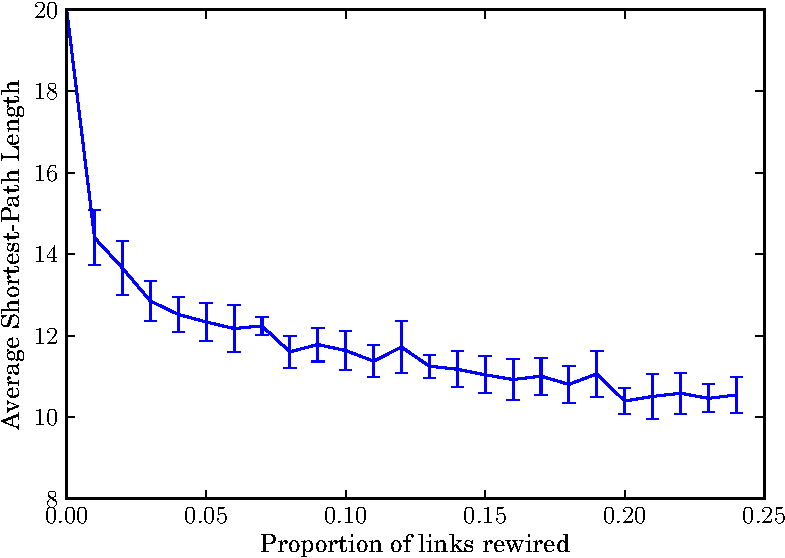
\includegraphics[width=0.7\textwidth]{figures/smallWorldTorus}
				\caption[Average shortest-path length for folded 40-ary 2-cube.]{Average
				shortest-path length for folded 40-ary 2-cube (mean of 10 runs, error
				bars show 1 standard deviation).}
				\label{fig:smallWorldTorus}
			\end{figure}
			
			This algorithm is readily extended to torus topologies similar to
			SpiNNaker's. In this preliminary work, a $k$-ary 2-cube (a two dimensional
			torus $k$ nodes long in each dimension) was used as the initial network as
			in figure \ref{fig:torusNetworkB0}.  Random permutations are introduced as
			in the Watts-Strogatz model resulting in a network such as figure
			\ref{fig:torusNetworkB01}. A $k$-ary $n$-cube has an average shortest path
			length of $\frac{nk}{4}$.  This is because a packet travels (on average,
			under uniform random traffic) $\frac{1}{4}$ of the way around each of the
			$n$, $k$-node-long dimensions. In the figure, that means the average path
			length is $\frac{2 \times 6}{4} = 3$. Experiments using a simple
			graph-based model were carried out to determine the effects of rewiring on
			shortest-path length.  For the rewired network, the average shortest path
			is reduced from 3 to 2.77 hops.  Further, this model was used to confirm
			findings by Shin et al.  \cite{shin11} who found an increase in bandwidth
			when even just a small number of links are rewired. Figure
			\ref{fig:smallWorldTorus} demonstrates that this effect also applies to
			latency.
			
			\begin{figure}
				\center
				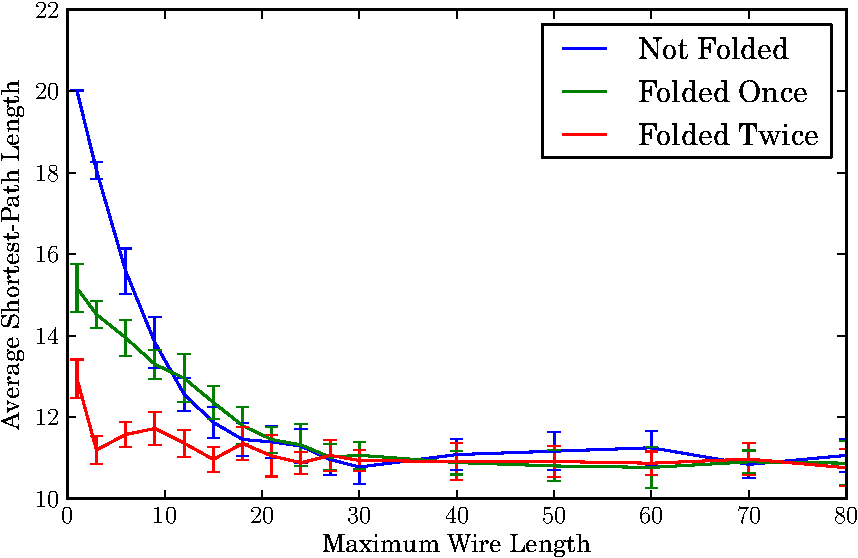
\includegraphics[width=0.7\textwidth]{figures/smallWorldLimitedWiring}
				\caption{Average shortest-path length for folded 40-ary 2-cube with 1\%
				rewiring}
				\label{fig:smallWorldLimitedWiring}
			\end{figure}
			
			Unfortunately, random links can be physically very long which, as
			described in the previous section, can cause problems for electrical
			high-speed serial links.  Though techniques exist to attempt to optimise
			the lay-out of networks containing random wiring \cite{koibuchi13}, these
			do not deal well with networks which also feature a large degree of
			regularity. An alternative approach is to simply limit the length of wires
			randomly inserted.  Unfortunately this fails to yield large reductions in
			path length in systems laid out na\"ively as in figure
			\ref{fig:torusNetwork}. If the network is folded as described in the
			previous section, however, significant reductions can be achieved. Figure
			\ref{fig:smallWorldLimitedWiring} shows the effect of rewiring 1\% of
			links when the maximum length of a randomly inserted wire is limited.  For
			networks folded twice (as in the case of the proposed SpiNNaker wiring
			plan), limiting wire length has little impact.
		
		\subsection{Further work}
			
			Figure \ref{fig:ringNetworkLimitedWires} shows valid random links in a
			small ring network if it were folded and random wires were limited to only
			short lengths. Nodes near the top and bottom of the ring potentially have
			shorter average path lengths compared with other nodes than nodes near the
			left and right of the ring. This is because the allowed links for top and
			bottom nodes connect nodes greater logical distances apart in the ring
			than those allowed on the left and right. The result is that the average
			path length from two different nodes becomes non-uniform across nodes in
			different parts of the system.
			
			\begin{figure}
				\center
				\begin{tikzpicture}[thick,inner sep=0.1cm]
	\foreach [count=\n] \t in {30,60,...,360}{
		\draw [help lines] (\t:2) -- (\t+30:2);
	}
	\foreach [count=\n] \t in {30,60,...,360}{
		\node [fill,circle] at (90-\t:2) (node \n) {};
	}
	
	\draw (node 8) to (node 10);
	\draw (node 8) to (node 11);
	
	\draw (node 7) to (node 11);
	\draw (node 7) to (node 12);
	
	\draw (node 6) to (node 12);
	\draw (node 6) to (node 1);
	
	\draw (node 5) to (node 1);
	\draw (node 5) to (node 2);
	
	\draw (node 4) to (node 2);
	
\end{tikzpicture}


				\caption[Valid random links in a folded ring network with short
				wires.]{Valid random links in ring network when folded and added wires
				limited to a length of 1 unit.}
				\label{fig:ringNetworkLimitedWires}
			\end{figure}
			
			The effect of this non-uniformity is yet to be studied. In addition, the
			magnitude of the differences in average path length in different parts of
			a network is reduced both in higher dimensional topologies and also after
			the network has been folded and mapped into physical racks and cabinets.
			Future work intends to implement a small-world style network both within
			the simulator described in the next section and, subsequently, within
			SpiNNaker's board-to-board links.
	
	
	\section{SpiNNaker network modelling}
		
		% Colaboration with others researching simulator platforms, due for journal
		% submission in coming months, final stages of writing. Context of the work:
		% want to try out modelling on different platforms. My contribution: some
		% writing and the development of an accurate software simulator for
		% SpiNNaker's interconnect. This work indirectly offers interesting insights
		% into behaviours due to the board-to-board links.
		
		A recent collaboration with other researchers within the department has
		investigated novel methods for high-level simulation and modelling of large
		scale systems. This work used SpiNNaker's interconnection network as its
		case study and included the development of a number of different simulators
		including both software and FPGA-based models. The work revealed that modern
		high-level languages for FPGA and hardware development, such as Bluespec
		System Verilog (BSV) \cite{nikhil04}, have reached a level of development
		efficiency comparable with software. This result demonstrates that modellers
		are no-longer faced with a decision of whether time allows for a hardware
		model but rather whether advantages of FPGA-based models, such as
		substantial simulation speed improvements, are desired over software based
		approaches.  The work is in its final draft and targeted for journal
		submission early in August this year.
		
		The author's primary contribution to this work has centred around the
		development of a detailed software model of SpiNNaker's interconnection
		network. In addition, a significant portion of the analysis of the
		simulators was also carried out. In this section, the simulator, named
		`Tickysim', is described below along with brief summary of results
		demonstrating faithfulness to the system it models. The section concludes
		with plans to use this simulator to guide future research.
		
		\subsection{Software simulator model}
			
			% Model 18 cores as traffic generators/consumers. Links are modelled as
			% delay elements (accurately captures req/ack links), internal arbitration
			% scheme is modelled along with pipelined router.
			
			\begin{figure}
				\begin{subfigure}[b]{0.65\textwidth}
					\center
					\tikzexternaldisable
					\begin{tikzpicture}[thick,remember picture,font=\small]
	
	\def\arbwidth{0.3cm}
	\def\arbheight{0.7cm}
	\def\arboffset{0.15cm}
	
	% An arbiter. Arguments:
	% 1: Name
	% 2: Node args
	% 3: Draw style
	\newcommand{\arb}[3]{
		\node (#1)
		      [minimum width=\arbwidth,minimum height=\arbheight, inner sep=0,#2]
		      {}
		      ;
		
		\coordinate (#1 in 1) at ($(#1.south west)!0.75!(#1.north west)$);
		\coordinate (#1 in 2) at ($(#1.south west)!0.25!(#1.north west)$);
		\coordinate (#1 out)  at (#1.east);
		
		\draw [#3]
		      (#1.south west)
		   -- (#1.north west)
		   -- ([yshift=-\arboffset]#1.north east)
		   -- ([yshift=\arboffset]#1.south east)
		   -- cycle
		      ;
	}
	
	% A buffer. Arguments:
	% 1: Name
	% 2: Node args
	% 3: Draw style
	% 4: Number of slots x
	% 5: Number of slots y
	\newcommand{\buf}[5]{
		\pgfmathsetlengthmacro{\bufsize}{0.2cm}
		\pgfmathsetlengthmacro{\width}{sqrt(#4)*\bufsize}
		\pgfmathsetlengthmacro{\height}{sqrt(#5)*\bufsize}
		\node (#1)
		      [ draw
		      , minimum width=\width
		      , minimum height=\height
		      , inner sep=0
		      , #2
		      , #3
		      ] { };
		
		% Draw Lines on buffers to indicate number of slots
		\foreach \x in {1,...,#4}{
			\ifthenelse{\not\equal{\x}{#4}}{
				\pgfmathsetmacro{\xx}{\x/#4}
				\draw [#3] ($(#1.south west)!\xx!(#1.south east)$)
				        -- ($(#1.north west)!\xx!(#1.north east)$);
			}{}
		}
		\foreach \y in {1,...,#5}{
			\ifthenelse{\not\equal{\y}{#5}}{
				\pgfmathsetmacro{\yy}{\y/#5}
				\draw [#3] ($(#1.south west)!\yy!(#1.north west)$)
				        -- ($(#1.south east)!\yy!(#1.north east)$);
			}{}
		}
		
		\coordinate (#1 in)  at (#1.west);
		\coordinate (#1 out) at (#1.east);
	}
	
	% A buffer-arbiter pair. Arguments:
	% 1: Name
	% 2: Arbiter node args
	% 3: Draw style
	% 4: Number of buffer slots x
	% 5: Number of buffer slots y
	\newcommand{\arbbuf}[5]{
		\arb{#1 arb}{#2}{#3}
		\buf{#1 buf}{right=\arbbufgap of #1 arb}{#3}{#4}{#5}
		\draw [#3] (#1 arb out) -- (#1 buf in);
	}
	
	% Draw a line with two bends. Arguments:
	% 1: Start
	% 2: End
	% 3: Draw style
	% 4: Bend 1 style
	% 5: Bend 2 style
	\newcommand{\drawbent}[5]{
		\draw [#3] (#1) #4 ($(#1)!0.5!(#2)$) #5 (#2);
	}
	
	\def\arbbufgap{0.1cm}
	\def\arbvgap{0.1cm}
	\def\arbhgap{0.4cm}
	
	\def\routerhgap{0.5cm}
	
	% Output Buffers. Arguments:
	% 1: Output name
	% 2: Line first bend y offset
	% 3: Line first bend x offset
	\newcommand{\outbuf}[3]{
		\path let \p1=(#1 buf in), \p2=([xshift=0.5*\routerhgap]router.east) in (\x2,\y1) coordinate (#1 out);
		\buf{#1 out buf}{right=\routerhgap of #1 out}{}{2}{1}
		\draw ($(router.north east)!#2!(router.south east)$)
		   -- ++(#3,0)
		   |- (#1 out buf)
		      ;
	}
	
	\def\packetgenvgap{0.6cm}
	
	% The node itself
	\node (model) [draw, rectangle, inner sep=0.25cm] {
		\begin{tikzpicture}[thick,remember picture]
			% Level 2
			\arbbuf{e ne}{}{}{1}{1}
			\buf{e  buf}{left=\arbbufgap of e ne arb in 1}{}{2}{1} \draw (e  buf) -- (e ne arb in 1);
			\buf{ne buf}{left=\arbbufgap of e ne arb in 2}{}{2}{1} \draw (ne buf) -- (e ne arb in 2);
			
			\arbbuf{n w}{below=\arbvgap of  e ne arb}{}{1}{1}
			\buf{n buf}{left=\arbbufgap of n w arb in 1}{}{2}{1} \draw (n buf) -- (n w arb in 1);
			\buf{w buf}{left=\arbbufgap of n w arb in 2}{}{2}{1} \draw (w buf) -- (n w arb in 2);
			\arbbuf{sw s}{below=\arbvgap of n w arb}{}{1}{1}
			\buf{sw buf}{left=\arbbufgap of sw s arb in 1}{}{2}{1} \draw (sw buf) -- (sw s arb in 1);
			\buf{s  buf}{left=\arbbufgap of sw s arb in 2}{}{2}{1} \draw (s  buf) -- (sw s arb in 2);
			\arbbuf{proc}{below=\arbvgap of sw s arb}{draw=white}{1}{1}
			
			% Level 1
			\arbbuf{e ne n w}{right=\arbhgap of $(e ne buf)!0.5!(n w buf)$}{}{1}{1}
			\drawbent{e ne buf out}{e ne n w arb in 1}{}{-|}{|-}
			\drawbent{n w buf out}{e ne n w arb in 2}{}{-|}{|-}
			\arbbuf{sw s proc}{right=\arbhgap of $(sw s buf)!0.5!(proc buf)$}{}{1}{1}
			\drawbent{sw s buf out}{sw s proc arb in 1}{}{-|}{|-}
			\coordinate (proc in) at  (sw s proc arb in 2);
			
			% Level 0 (root)
			\arbbuf{root}{right=\arbhgap of $(e ne n w buf)!0.5!(sw s proc buf)$}{}{2}{1}
			\drawbent{e ne n w buf out}{root arb in 1}{}{-|}{|-}
			\drawbent{sw s proc buf out}{root arb in 2}{}{-|}{|-}
			
			% Router
			\def\routerstages{4}
			\node (router)
			      [inner ysep=0.5cm,inner xsep=1em,draw, rectangle, right=\arbbufgap of root buf out]
			      {Router}
			      ;
			\draw (root buf out) -- (router.west);
			
			% Router pipeline stage divisions
			\begin{scope}
				\clip       ($(router.south west)!0.0!(router.north west)$)
				  rectangle ($(router.south east)!0.2!(router.north east)$)
				            ($(router.south west)!0.8!(router.north west)$)
				  rectangle ($(router.south east)!1.0!(router.north east)$)
				  ;
				
				\foreach \x in {2,...,\routerstages}{
					\pgfmathsetmacro{\xx}{(\x-1)/\routerstages}
					\draw  ($(router.south west)!\xx!(router.south east)$)
					    -- ($(router.north west)!\xx!(router.north east)$);
				}
			\end{scope}
			
			\outbuf{e}{ 0.2}{0.3*\routerhgap + 0.1cm}
			\outbuf{ne}{0.3}{0.3*\routerhgap + 0.2cm}
			\outbuf{n}{ 0.4}{0.3*\routerhgap + 0.3cm}
			\outbuf{w}{ 0.5}{0.3*\routerhgap + 0.4cm}
			\outbuf{sw}{0.6}{0.3*\routerhgap + 0.3cm}
			\outbuf{s}{ 0.7}{0.3*\routerhgap + 0.2cm}
			
			% Packet Generator
			\node (packet gen)
			      [below=\packetgenvgap of sw s proc arb in 2, xshift=-0.5*\arbhgap]
			      [draw, rectangle, text width = 2cm, align=center, inner sep=0.2cm]
			      {Packet Generator}
			    ;
			
			\buf{packet gen buf}{above=\arbbufgap of packet gen.north}{}{1}{2}
			\draw (packet gen buf.north) |- (sw s proc arb in 2);
			\draw (packet gen.north) -- (packet gen buf.south);
			
			% Packet Consumer
			\path let \p1=(router.south)
			        , \p2=(packet gen.north)
			      in coordinate (packet con north) at (\x1,\y2);
			\node (packet con)
			      [below=0 of packet con north,xshift=0.7cm]
			      [draw, rectangle, text width = 2cm, align=center, inner sep=0.2cm]
			      {Packet Consumer}
			    ;
			\draw ($(router.north east)!0.8!(router.south east)$)
			   -- ++(0.3*\routerhgap + 0.1cm, 0)
			      coordinate (packet con router output)
			    ;
			\path let \p1=(packet con router output)
			        , \p2=(packet con.north)
			      in coordinate (packet con input) at (\x1,\y2);
			\buf{packet con buf}{above=\arbbufgap of packet con input}{}{1}{2}
			\draw (packet con input) -- (packet con buf.south);
			\draw (packet con router output) -- (packet con buf.north);
			
		\end{tikzpicture}
	};
	
	
	\def\keyentrygap{1.5em}
	\def\keylabelgap{0.3cm}
	
	% The Key
	\node [below=0.5cm of model, inner sep=0] {
		\begin{tikzpicture}[thick,remember picture]
			
			\arb{key arb}{}{}
			\node (key arb label) [right=\keylabelgap of key arb] {Round-Robin Arbiter};
			
			\buf{key buf}{right=\keyentrygap of key arb label}{}{1}{1}
			\node (key buf label) [right=\keylabelgap of key buf] {Buffer};
			
			\node [left=\keyentrygap of key arb] {Key:};
		\end{tikzpicture}
	};
	
	
	\def\inpindist{0.75cm}
	\def\outpindist{0.8cm}
	
	% XXX: Note that the text here differs from the labelling used internally.
	% This is due to the fact that the original assignment was discovered to be
	% erroneuous and just correcting the text was easier than replacing
	% everything.
	
	% Input pins
	\draw (e  buf in) -- ++(-\inpindist,0) node [left] {E};
	\draw (ne buf in) -- ++(-\inpindist,0) node [left] {S};
	\draw (n  buf in) -- ++(-\inpindist,0) node [left] {NE};
	\draw (w  buf in) -- ++(-\inpindist,0) node [left] {N};
	\draw (sw buf in) -- ++(-\inpindist,0) node [left] {W};
	\draw (s  buf in) -- ++(-\inpindist,0) node [left] {SW};
	
	% Output pins
	\draw (e  out buf out) -- ++(\outpindist,0) node [right] {E};
	\draw (ne out buf out) -- ++(\outpindist,0) node [right] {S};
	\draw (n  out buf out) -- ++(\outpindist,0) node [right] {NE};
	\draw (w  out buf out) -- ++(\outpindist,0) node [right] {N};
	\draw (sw out buf out) -- ++(\outpindist,0) node [right] {W};
	\draw (s  out buf out) -- ++(\outpindist,0) node [right] {SW};
	
\end{tikzpicture}

					\caption{Model of a SpiNNaker chip. A packet generator and consumer
					model SpiNNaker's eighteen cores. A tree of packet arbiters mimmicing
					SpiNNaker's Network on Chip (NoC) feeds a stream of packets into a
					router model.}
					\label{fig:tickysim-model-chip}
				\end{subfigure}
				~~~~~
				\begin{subfigure}[b]{0.28\textwidth}
					\centering
					% A diagram showing links delays between nodes.
\begin{tikzpicture}[thick,font=\small]
	
	\def\nodesize{1.0cm}
	\def\scale{2.1}
	
	\begin{scope}[scale=\scale]
		\clip (-0.85,-0.85) rectangle ( 0.85, 0.85);
		
		\foreach \x in {-1,...,1}{
			\foreach \y in {-1,...,1}{
				\node [ draw
				      , rectangle
				      , minimum width=\nodesize
				      , minimum height=\nodesize
				      , inner sep=0
				      ]
				      (node \x\y)
				      at (\x,\y)
				      {};
			}
		}
	\end{scope}
	
	\newcommand{\link}[2]{
		\draw (#1) to (#2);
		\node [ draw
		      , fill=white
		      , rectangle
		      , inner sep=0.1cm
		      ]
		      at ($(#1)!0.5!(#2)$)
		      {D};
	}
	
	% Links from the central node outward
	\foreach \x/\y in {1/0, 0/1, 1/1, -1/0, 0/-1, -1/-1}{
		\link{node 00}{node \x\y}
	}
	% Other visible links (not the central node)
	\link{node 0-1}{node 10}
	\link{node -10}{node 01}
	
\end{tikzpicture}

					\vspace{1.8cm}
					
					\caption{Delay elements inserted between chips model the effects of
					link latency.}
					\label{fig:tickysim-model-link-delays}
				\end{subfigure}
				
				\caption{The Tickysim simulator model.}
				\label{fig:tickysim-model}
			\end{figure}
			
			The basic unit of the Tickysim simulator model is a high-level model of a
			single SpiNNaker chip which is summarised in figure
			\ref{fig:tickysim-model-chip}. Since the model focuses on the
			interconnection network, the eighteen processors present on a SpiNNaker
			chip are instead modelled by a simple packet generator and consumer. This
			simplification saves a large amount of simulation overhead at the expense
			of detail in processor behaviour. Since the exact computation performed is
			not the focus of the model, this simplification should significantly
			impact results.
			
			The model captures the basic structure of the Network-on-Chip (NoC) within
			SpiNNaker chips. In particular, streams of packets incident on the chip
			are merged using a tree of mergers before entering a model of the on-chip
			router. The simulated router models a multiple stage pipeline matching
			that of the actual SpiNNaker router along with packet dropping and other
			behaviours.
			
			The complete model consists of a network of these chip models
			interconnected by delay elements as illustrated in figure
			\ref{fig:tickysim-model-link-delays}.  These delay elements model the
			latency introduced when packets cross a chip-to-chip boundary.
			
			The model is extensively instrumented and configurable to allow a range of
			metrics to be collected and numerous parameters such as buffer sizes,
			injected traffic patterns and router behaviour to be modified. In
			addition, the software architecture is structured to allow straightforward
			extension making it suitable for use in later work.
			
			When configured to model a 144-chip SpiNNaker system, the model runs
			around 7,000 times slower than real time on an Intel Xeon E3-1225 V2
			running at 3.2 GHz with 32 GB of RAM, the same order of magnitude
			slow-down experienced by comparable software simulators such as INSEE
			\cite{navaridas11insee}. Though the model itself is single threaded,
			parameter-sweep style experiments may be performed in parallel using
			commodity compute resources. Experiments conducted using idle department
			workstations allowed hundreds of parameter settings to be tested in the
			time required to run a single experiment on a single machine.
		
		\subsection{Results}
			
			% Experiments performed showed highly matched behaviour between the model
			% and SpiNNaker but reveal the effects of the non-homogeneity introduced
			% by board-to-board links for certain traffic patterns.
			
			Experiments were carried out to verify that the simulators bore a close
			resemblance to the actual SpiNNaker hardware. These consisted of injecting
			a selection of synthetic traffic patterns at various injection rates and
			monitoring standard metrics such as number of packets dropped and accepted
			load (number of packets arriving at their destination).
			
			\begin{figure}
				\begin{subfigure}{\textwidth}
					% Commands for producing plots as used in the paper.

% Plot an accepted/dropped packet load graph
% Arguments:
%  #1: Number of nodes in the system
%  #2: Traffic pattern name
\newcommand{\plotresults}[2]{%
	\begin{tikzpicture}
		\newcommand{\width}{0.48\textwidth}
		\newcommand{\height}{5.5cm}
		
		%\selectcolormodel{gray};
		
		\begin{axis}[ xlabel=Injection Rate
		            , ylabel=Accepted Load
		            , xmin=0, xmax=1
		            , ymin=0
		            , width=\width
		            , height=\height
		            , yticklabel style = { /pgf/number format/precision=1
		                                 , /pgf/number format/fixed
		                                 , /pgf/number format/fixed zerofill
		                                 }
		            ]
			\addplot+ table [x=injection_rate, y=accepted_load] {results/#1_spinnaker_#2.csv};
			\addplot+ table [x=injection_rate, y=accepted_load] {results/#1_tickysim_#2.csv};
		\end{axis}
		
		\begin{axis}[ xshift=\width+0.2cm
		            , xlabel=Injection Rate
		            , ylabel=Dropped Packets
		            , xmin=0, xmax=1
		            , ymin=0
		            , width=\width
		            , height=\height
		            %, yticklabel pos=right
		            , yticklabel style = { /pgf/number format/precision=1
		                                 , /pgf/number format/fixed
		                                 , /pgf/number format/fixed zerofill
		                                 }
		            , legend pos=south east
		            , legend entries = { SpiNNaker
		                               , Tickysim
		                               }
		            ]
			\addplot+ table [x=injection_rate, y=dropped] {results/#1_spinnaker_#2.csv};
			\addplot+ table [x=injection_rate, y=dropped] {results/#1_tickysim_#2.csv};
		\end{axis}
	\end{tikzpicture}%
}

					\plotresults{144}{cyclic}
					
					\caption{`Uniform' traffic.}
					\label{fig:results-144-accuracy-cyclic}
				\end{subfigure}
				
				\vspace{1em}
				
				\begin{subfigure}{\textwidth}
					% Commands for producing plots as used in the paper.

% Plot an accepted/dropped packet load graph
% Arguments:
%  #1: Number of nodes in the system
%  #2: Traffic pattern name
\newcommand{\plotresults}[2]{%
	\begin{tikzpicture}
		\newcommand{\width}{0.48\textwidth}
		\newcommand{\height}{5.5cm}
		
		%\selectcolormodel{gray};
		
		\begin{axis}[ xlabel=Injection Rate
		            , ylabel=Accepted Load
		            , xmin=0, xmax=1
		            , ymin=0
		            , width=\width
		            , height=\height
		            , yticklabel style = { /pgf/number format/precision=1
		                                 , /pgf/number format/fixed
		                                 , /pgf/number format/fixed zerofill
		                                 }
		            ]
			\addplot+ table [x=injection_rate, y=accepted_load] {results/#1_spinnaker_#2.csv};
			\addplot+ table [x=injection_rate, y=accepted_load] {results/#1_tickysim_#2.csv};
		\end{axis}
		
		\begin{axis}[ xshift=\width+0.2cm
		            , xlabel=Injection Rate
		            , ylabel=Dropped Packets
		            , xmin=0, xmax=1
		            , ymin=0
		            , width=\width
		            , height=\height
		            %, yticklabel pos=right
		            , yticklabel style = { /pgf/number format/precision=1
		                                 , /pgf/number format/fixed
		                                 , /pgf/number format/fixed zerofill
		                                 }
		            , legend pos=south east
		            , legend entries = { SpiNNaker
		                               , Tickysim
		                               }
		            ]
			\addplot+ table [x=injection_rate, y=dropped] {results/#1_spinnaker_#2.csv};
			\addplot+ table [x=injection_rate, y=dropped] {results/#1_tickysim_#2.csv};
		\end{axis}
	\end{tikzpicture}%
}

					\plotresults{144}{complement}
					
					\caption{`Complement' traffic.}
					\label{fig:results-144-accuracy-complement}
				\end{subfigure}
				
				\caption[Packet acceptance and dropping in SpiNNaker
				and TIckysim.]{Comparison of accepted load and dropping rates in
				SpiNNaker and Tickysim. A load of 1.0 is equal to the bandwidth
				available across a single link. Packet dropping rates are as a
				proportion of the number of packets injected.}
				\label{fig:results-144-accuracy}
			\end{figure}
			
			Figure \ref{fig:results-144-accuracy-cyclic} gives a representative
			example of the results obtained. In this example, a `uniform' traffic
			pattern was used where nodes produce traffic destined for each node in the
			system in turn. Both SpiNNaker and the Tickysim model exhibit classic
			behaviour for this pattern with all traffic being accepted until a point
			when the network saturates.  Beyond this saturation point, packets are
			dropped. Since packets are dropped after a fixed timeout, this increases
			the time between sending of packets and thus causes the accepted load to
			drop to far below the rate immediately prior to saturation.
			
			\begin{figure}
				\center
				% Comparison of three heatmaps of SpiNNaker's complement traffic pattern.
\begin{tikzpicture}[baseline]
	% Produce a single heatmap for comparison of the SpiNNaker complement traffic
	% pattern.
	% Arguments:
	%  #1: The injection rate
	%  #2: Extra arguments for the axis environment
	%  #3: Title
	\newcommand{\spinncomplementheatmap}[3]{
		\begin{axis}[ xlabel=X
		            , title={#3}
		            , title style={align=center}
		            , axis equal=true
		            , colorbar style={ ylabel={Packets Dropped}
		                             , yticklabel pos = left
		                             , yticklabel style = { /pgf/number format/precision=3
		                                                  , /pgf/number format/fixed
		                                                  , /pgf/number format/fixed zerofill
		                                                  }
		                             }
		            , colormap={blackwhite}{rgb=(0,0,0); rgb=(1,1,1)}
		            , view={0}{90}
		            , xmin=-0.5, xmax=11.5
		            , ymin=-0.5, ymax=11.5
		            , point meta min=0, point meta max=0.018
		            , xtick={0,3,...,11}
		            , ytick={0,3,...,11}
		            , minor tick num=2
		            , #2
		            ]
			\addplot3 [ surf
			          , shader=flat corner
			          ] table [ x expr={\thisrow{chip_x}-0.5}
			                  , y expr={\thisrow{chip_y}-0.5}
			                  , z expr={\thisrow{dumped} / 1200000}
			                  ] {results/SpiNNaker_complement_#1.csv}
			          ;
			\addplot+ [ no markers
			          , gray
			          , ultra thick
			          ] table {results/threeboard_outline.csv}
			          ;
		\end{axis}
	}
	
	\newcommand{\stdwidth}{0.27\textwidth}
	\newcommand{\stdoffset}{(\stdwidth-0.50cm)}
	
	\spinncomplementheatmap{0.10}{ width = \stdwidth
	                             , height = \stdwidth
	                             , xshift=0*\stdoffset
	                             , ylabel=Y
	                             }{Before saturation}
	\spinncomplementheatmap{0.30}{ width = \stdwidth
	                             , height = \stdwidth
	                             , xshift=1*\stdoffset
	                             , yticklabel={$ $}
	                             }{Semi-saturated}
	\spinncomplementheatmap{0.40}{ width = \stdwidth
	                             , height = \stdwidth
	                             , xshift=2*\stdoffset
	                             , yticklabel={$ $}
	                             , colorbar
	                             , colorbar style={xshift=1.3cm}
	                             }{Fully saturated}
\end{tikzpicture}

				\caption[Packet dropping in a three board SpiNNaker machine.]{Packet
				dropping in a three board SpiNNaker machine under complement traffic at
				various injection rates. Thick lines show boundaries between boards in
				the system.}
				\label{fig:heatmap-spinnaker-complement}
			\end{figure}
			
			Some traffic patterns such as `complement', however, exhibited artefacts
			in SpiNNaker due to the prototype implementation of the HSS links between
			boards not being able to achieve full bandwidth. Since the difference due
			to these links is not modelled by Tickysim, their results clearly differ.
			Figure \ref{fig:results-144-accuracy-complement} demonstrates this effect
			in the form of two distinct phases of saturation in SpiNNaker but just one
			in Tickysim. In complement traffic, several distinct clusters of
			communicating nodes occur in the network. In SpiNNaker, those clusters
			which span board boundaries saturate first due to their lower bandwidth
			followed later by the native chip-to-chip links. This behaviour can be
			seen in \ref{fig:heatmap-spinnaker-complement} where there is a phase of
			packets being dropped in only certain parts of the network (a sign of
			saturation in those areas).
		
		\subsection{Further work}
			
			% Plans to include models of SpiNNaker links. Preliminary trials at
			% accurately modelling these have been unsuccessful. Will be used to guide
			% work on these links.
			
			Work is planned to more accurately model the behaviour of board-to-board
			links within Tickysim to allow its use in evaluating the utility of small
			world connectivity. Preliminary attempts to model board-to-board links as
			simply having longer latencies have been unsuccessful. It is suspected
			that the mechanisms used within the HSS links must also be modelled to
			match SpiNNaker's behaviour.
	
	
	\section{SpiNNaker FPGA connectivity}
		
		% Work started at CapoCaccia with input from various parties to get
		% SpiNNaker peripherals working. The start of a project to get peripherals
		% properly integrated and generally add some routing smarts to the FPGAs
		
		At the 2014 Capo Caccia Neuromorphic Workshop a group was formed to discuss
		requirements for extending the HSS links available within SpiNNaker for
		connecting peripherals and to host computers. In particular, the group was
		interested in the acceleration of the loading of neural models and
		extraction of results.  As a result of these discussions, work began to
		extend the existing infrastructure used for board-to-board links to support
		flexible additional connectivity. This work has concentrated on the
		development of FPGA designs to support tasks such as routing packets to and
		from peripherals and hosts and the integration of HSS links operating at
		different speeds.
		
		This section outlines the existing infrastructure for board-to-board links
		followed by a description of the extensions developed and how they address
		the requirements proposed at the workshop. The section concludes with
		planned future work which builds on the infrastructure developed.
		
			\subsection{Existing infrastructure}
				
				% Description of what exists already in the board-to-board links,
				% outline the protocol's principles. Also describe the rdy/vld
				% interface.
				
				\begin{figure}
					\center
					\begin{tikzpicture}[thick]
	\def\twoofsevenheight{1.0em}
	\def\twoofsevensep{1.5em}
	
	\def\bordersep{1.0em}
	
	% 2-of-7 link handlers
	\foreach \row in {0,...,7}{
		\node [ draw
		      , rectangle
		      , yshift=\row*\twoofsevensep
		      , inner sep=0.3em
		      , minimum height=\twoofsevenheight
		      ]
		      (two of seven \row)
		      {\tiny{2 of 7}};
	}
	
	% Framing block
	\node [ draw
	      , rectangle
	      , right=of $(two of seven 0.east)!0.5!(two of seven 7.east)$
	      , minimum height = 7*\twoofsevensep + \twoofsevenheight
	      , text width=2.5cm
	      , align=center
	      ]
	      (framing)
	      {Framing and Reliability};

	% Links from 2-of-7 to framing
	\foreach \row in {0,...,7}{
		\draw [<->]
		      (two of seven \row.east)
		   -- (two of seven \row.east -| framing.west)
		    ;
	}
	
	% Links from 2-of-7 to chips
	\foreach \row in {0,...,7}{
		\draw [<->]
		      (two of seven \row.west)
		   -- ++(-1cm,0) coordinate (two of seven wire \row)
		    ;
	}
	
	% GTP
	\node [ draw
	      , rectangle
	      , right=of framing
	      , minimum height = 7*\twoofsevensep + \twoofsevenheight
	      , text width=2.5cm
	      , align=center
	      ]
	      (gtp)
	      {Gigabit Transceiver\\(Hard IP)};
	
	% Framing to/from GTP wires
	\draw [<->] (framing.east) -- (gtp.west);
	
	% Gigabit links
	\draw [<->] (gtp.east) -- ++(1cm,0) coordinate (gtp wire);
	
	% FPGA Border
	\draw ([shift={(-\bordersep,-\bordersep)}]two of seven 0.south west)
	      rectangle
	      ([shift={( \bordersep, \bordersep)}]gtp.north east);
	
	% Chip label
	\node [ left=0 of $(two of seven wire 0)!0.5!(two of seven wire 7)$
	      , rotate=90
	      , anchor=south
	      ]
	      {SpiNNaker Chip Links};
	
	% HSS link label
	\node [ right=0 of gtp wire
	      , rotate=90
	      , anchor=north
	      ]
	      {S-ATA connector};
\end{tikzpicture}

					
					\caption[Existing board-to-board link FPGA design.]{Existing
					board-to-board link FPGA design. Each FPGA contains two independent
					copies of this design so that the three FPGAs on each board can
					implement all six board-to-board links.}
					\label{fig:existing-fpga-links}
				\end{figure}
				
				The existing board-to-board links are implemented within the FPGAs on
				each SpiNNaker board. Each HSS link is designed to transparently replace
				eight chip-to-chip SpiNNaker links. The design, as shown in figure
				\ref{fig:existing-fpga-links} contains three basic elements. A 2-of-7
				block translates between the asynchronous 2-of-7 protocol used by
				SpiNNaker chip links and a synchronous protocol used within the FPGA
				design. The next block assembles and disassembles `frames' containing
				SpiNNaker packets and ensures reliable communication by verifying
				incoming frames and retransmitting frames if required. The final block
				is provided as `hard IP' by the FPGA manufacturer rather than soft
				programmable FPGA logic to enable it to run at the high speeds required
				serialisation and deserialisation of frames for the HSS link.
				
				\begin{figure}
					\center
					\begin{tikzpicture}[thick]
						\input{|"wavedromtikz.py wavedrom figures/rdyvld-protocol.drom"}
					\end{tikzpicture}
					
					\caption{Example of the ready/valid protocol.}
					\label{fig:rdyvld-protocol}
				\end{figure}
				
				Within and between blocks, data is transferred using a simple
				point-to-point `ready/valid' protocol illustrated in figure
				\ref{fig:rdyvld-protocol}.  The receiever asserts a `ready' signal
				whenever it is able to accept new data. The sender places data it wishes
				to send on a data bus while asserting a `valid' signal. If the valid and
				ready signals are simultaneously asserted on the rising edge of the
				clock, the data is considered received. This protocol allows a value to
				be transmitted up-to every clock cycle while still allowing both the
				sender and receiver control over the rate that data flows.
			
			\subsection{Proof-of-concept I/O device}
				
				% Describe principle of how a router will be integrated and streams
				% merged.
				
				To enable extension of the existing board-to-board system for other
				purposes, the ready/valid protocol described previously, has been
				standardised for communication between new blocks. Additionally the
				standard dictates that the bus should be able to carry a complete 72-bit
				SpiNNaker packet each cycle.
				
				\begin{figure}
					\center
					\begin{tikzpicture}[thick]
	\def\twoofsevenheight{1.0em}
	\def\twoofsevensep{1.5em}
	
	\def\bordersep{1.0em}
	
	% Router
	\node [ draw
	      , rectangle
	      , anchor=north west
	      , minimum height = 1cm + 7*\twoofsevensep + \twoofsevenheight
	      , text width=1.5cm
	      , align=center
	      ]
	      (router)
	      {Router};
	
	% Framing blocks
	\node [ draw
	      , rectangle
	      , right=of router.north east
	      , anchor = north west
	      , minimum height = 3.5*\twoofsevensep + 0.5*\twoofsevenheight
	      , text width=2.5cm
	      , align=center
	      ]
	      (framing)
	      {Framing and Reliability};
	\node [ draw
	      , rectangle
	      , below=of framing
	      , minimum height = 3.5*\twoofsevensep + 0.5*\twoofsevenheight
	      , text width=2.5cm
	      , align=center
	      ]
	      (framing periph)
	      {Framing and Reliability};
	
	% 2-of-7 link handlers
	\foreach \row [count=\i from 0] in {-3.5,...,3.5}{
		\node [ draw
		      , rectangle
		      , yshift=\row*\twoofsevensep
		      , inner sep=0.3em
		      , minimum height=\twoofsevenheight
		      , left= of router.west
		      ]
		      (two of seven \i)
		      {\tiny{2 of 7}};
	}

	% Links from 2-of-7 to router
	\foreach \row in {0,...,7}{
		\draw [<->]
		      (two of seven \row.east)
		   -- (two of seven \row.east -| router.west)
		    ;
	}

	% Links from router to b2b framing
	\foreach \row in {-3.5,...,3.5}{
		\draw [<->]
		      ([yshift=-0.7em*\row]framing.west -| router.east)
		   -- ([yshift=-0.7em*\row]framing.west)
		    ;
	}
	
	% Links from router to periph framing
	\foreach \row in {-3.5,...,3.5}{
		\draw [<->]
		      ([yshift=-0.7em*\row]framing periph.west -| router.east)
		   -- ([yshift=-0.7em*\row]framing periph.west)
		    ;
	}
	
	% Links from 2-of-7 to chips
	\foreach \row in {0,...,7}{
		\draw [<->]
		      (two of seven \row.west)
		   -- ++(-1cm,0) coordinate (two of seven wire \row)
		    ;
	}
	
	% GTPs
	\node [ draw
	      , rectangle
	      , right=of framing
	      , minimum height = 3.5*\twoofsevensep + 0.5*\twoofsevenheight
	      , text width=2.5cm
	      , align=center
	      ]
	      (gtp)
	      {Gigabit Transceiver\\(Hard IP)};
	\node [ draw
	      , rectangle
	      , below=of gtp
	      , minimum height = 3.5*\twoofsevensep + 0.5*\twoofsevenheight
	      , text width=2.5cm
	      , align=center
	      ]
	      (gtp periph)
	      {Gigabit Transceiver\\(Hard IP)};
	
	% Framing to/from GTP wires
	\draw [<->] (framing.east)        -- (gtp.west);
	\draw [<->] (framing periph.east) -- (gtp periph.west);
	
	% Gigabit links
	\draw [<->] (gtp.east)        -- ++(1cm,0) coordinate (gtp wire);
	
	% FPGA Border
	\draw ([shift={(-\bordersep, \bordersep)}]router.north -| two of seven 7.west)
	      rectangle
	      ([shift={( \bordersep,-\bordersep)}]gtp periph.south east);
	
	% Chip label
	\node [ left=0 of $(two of seven wire 0)!0.5!(two of seven wire 7)$
	      , rotate=90
	      , anchor=south
	      ]
	      (spinnaker chip links label)
	      {SpiNNaker Chip Links};
	
	% HSS link label
	\node [ right=0 of gtp wire
	      , rotate=90
	      , anchor=north
	      ]
	      {Board-to-Board};
	
	
	%%%%%%%%%%%%%%%%%%%%%%%%%%%%%%%%%%%%%%%%%%%%%%%%%%%%%%%%%%%%%%%%%%%%%%%%%%%%%%%%
	% Peripheral
	%%%%%%%%%%%%%%%%%%%%%%%%%%%%%%%%%%%%%%%%%%%%%%%%%%%%%%%%%%%%%%%%%%%%%%%%%%%%%%%%
	
	
	% Framing block
	\node [ draw
	      , rectangle
	      , below=1.5cm of framing periph
	      , minimum height = 3.5*\twoofsevensep + 0.5*\twoofsevenheight
	      , text width=2.5cm
	      , align=center
	      ]
	      (framing device)
	      {Framing and Reliability};
	
	% UART block
	\node [ draw
	      , rectangle
	      , left = of framing device.south west
	      , anchor = south east
	      , minimum height = 1.8em
	      , text width=1.5cm
	      , align=center
	      ]
	      (uart)
	      {UART};
	
	
	% Links from UART to b2b framing
	\foreach \row in {-3.5,...,2.5}{
		\draw [<->]
		      ([yshift=-0.7em*\row]framing device.west)
		   -- ++(-0.5cm,0)
		      node [xshift=-0.5ex] {$\times$}
		    ;
	}
	\draw [<->]
	      ([yshift=-0.7em*3.5]framing device.west)
	   -- ([yshift=-0.7em*3.5]uart.east |- framing device.west)
	    ;
	
	% GTP
	\node [ draw
	      , rectangle
	      , below=1.5cm of gtp periph
	      , minimum height = 3.5*\twoofsevensep + 0.5*\twoofsevenheight
	      , text width=2.5cm
	      , align=center
	      ]
	      (gtp device)
	      {Gigabit Transceiver\\(Hard IP)};
	
	% Framing to/from GTP wires
	\draw [<->] (framing device.east) -- (gtp device.west);
	
	% Gigabit links
	\draw [<->]
	      (gtp periph.east)
	   -- ++(1cm,0)
	   |- (gtp device.east);
	
	% FPGA Border
	\draw ([shift={(-\bordersep, \bordersep)}]uart.west |- framing device.north)
	      rectangle
	      ([shift={( \bordersep,-\bordersep)}]gtp device.south east);
	
	% Link to USB
	\draw [<->] (uart.west) -- ++(-1cm,0) coordinate (uart connection);
	
	\node [left=0 of uart connection] {Host PC};
	
	
	
	
	\draw [decorate,decoration={brace,amplitude=1em,raise=1ex}]
	      ([shift={(0,-\bordersep)}]spinnaker chip links label.north |- router.south)
	   -- coordinate (spinnaker label)
	      ([shift={(0, \bordersep)}]spinnaker chip links label.north |- router.north);
	
	\draw [decorate,decoration={brace,amplitude=1em,raise=1ex}]
	      ([shift={(0,-\bordersep)}]spinnaker chip links label.north |- uart.south)
	   -- coordinate (periph label)
	      ([shift={(0, \bordersep)}]spinnaker chip links label.north |- framing device.north);
	
	\node [left=1.5em of spinnaker label, rotate=90, anchor=south] {SpiNNaker FPGA};
	\node [left=1.5em of periph label, rotate=90, anchor=south] {Raggedstone 2};
	
	
\end{tikzpicture}

					
					\caption[Proof-of-concept low-speed I/O system.]{Proof-of-concept
					low-speed I/O system. A spare HSS link from an FPGA on a SpiNNaker
					board connects to a Raggedstone 2 board connected to a host PC.}
					\label{fig:proof-of-concept-fpga-links}
				\end{figure}
				
				Based on the ready/valid standard, a number of basic components, such as
				simple routers, for extending the existing design were produced. Using
				these components, a simple proof of concept low-speed host connection
				was developed to allow injection and extraction of packets directly into
				the network. In this system, which is sketched in figure
				\ref{fig:proof-of-concept-fpga-links}, a SpiNNaker board is connected to
				an off-the-shelf Raggedstone 2 FPGA development baord
				\cite{raggedstone2} using an unused S-ATA connector on the SpiNNaker
				board. A host PC then connects to the Raggedstone 2 via an onboard FTDI
				USB-to-UART (Universal Asynchronous Receiver/Transmitter) converter
				providing a simple to drive but low speed (2.3 Mbit/s) compared to the
				HSS link (1.5 Gbits/s) connection over which SpiNNaker packets can be
				transmitted to and from the host.
				
				A router is used on the SpiNNaker boards' FPGAs to route packets from
				incoming SpiNNaker chips either along their usual board-to-board
				connection, to the Raggedstone 2 board or both.  Packets are routed
				using the same key and mask mechanism described in
				\S\ref{sec:spinn-router} though in the current, preliminary design the
				routing table contains only a single entry.  Packets routed to the
				Raggedstone 2 board the same HSS link protocol as board-to-board links
				to travel to and from the Raggedstone 2 board.  On the Raggedstone 2,
				one of the eight streams of packets is fed to a UART block which uses a
				simple protocol to send and receive SpiNNaker packets at low speed to a
				host PC. The UART connection to the host is the bottleneck in the system
				and more performant technologies such as USB 3.0 would instantly enable
				greater performance. With this bottleneck removed the only overhead is
				an additional 13 ns of latency added by the router and throughput would
				be unaffected.
				
				This proof-of-concept device has been successfully integrated into the
				SpiNNaker implementation of Nengo where it can be used to transmit
				values in to and out of a model in real time. Despite its low bandwidth,
				the link carries raw SpiNNaker packets performs favourably compared to
				the previous Ethernet implementation whose large protocol overheads
				resulted in very low bandwidth.
			
			\subsection{Further work}
				
				% Next steps will involve getting basic routing up and running, then on
				% to my planned project, see next chapter.
				
				With the basic infrastructure in place for implementing custom routing
				schemes and using additional HSS links within SpiNNaker's FPGAs in
				place, it is now possible to develop high speed peripheral and host
				connectivity. In addition, this infrastructure allows for the addition
				of axillary links between boards which could be used for the
				implementation of small-world network connectivity.
				
				In collaboration with researchers at the Technical University of Munich,
				a small board containing an FPGA with both a HSS link and a USB 3.0 link
				is being developed. This board's FPGA could be loaded with a design very
				similar to that used in the Raggedstone 2 but with the UART block
				replaced with a USB 3.0 block. Using this board, it is hoped that high
				bandwidth communication between a host and SpiNNaker machine should
				become possible. As well as improving system performance this will also
				enable greater visibility of SpiNNaker's network behaviour which may
				prove valuable in later work.

